\documentclass[10pt,twocolumn]{scrartcl}

\usepackage[utf8]{inputenc}
\usepackage[T1]{fontenc}
\usepackage[ngerman]{babel}

\usepackage{lmodern}
\usepackage[sc]{mathpazo} % or option osf
\usepackage{newpxmath}
\usepackage[scaled = 0.85]{beramono}

\usepackage{xpatch}
\usepackage{xcolor}
\usepackage{realboxes}
\definecolor{mygray}{rgb}{0.9,0.9,0.9}
\usepackage{listings}
\usepackage{pmboxdraw}
\lstdefinelanguage{commentonly}{ morecomment=[l]{\#} }
\lstset{literate=%
{μ}{{$\mu$}}1
{Ö}{{\"O}}1
{Ä}{{\"A}}1
{Ü}{{\"U}}1
{ß}{{\ss}}1
{ü}{{\"u}}1
{ä}{{\"a}}1
{ö}{{\"o}}1
{α}{{$\alpha$}}1
{λ}{{$\lambda$}}1
{├}{{\textSFviii}}1
{─}{{\textSFx}}1
{└}{{\textSFii}}1
{×}{{\texttimes}}1
,basicstyle=\ttfamily
,backgroundcolor=\color{mygray}
,commentstyle=\emph
,language=commentonly
,upquote=true
}
\makeatletter
\xpretocmd\lstinline{\Colorbox{mygray}\bgroup\appto\lst@DeInit{\egroup}}{}{}
\makeatother

\usepackage{enumitem}

\usepackage{adjustbox}
\usepackage[a4paper, margin=1mm, includefoot, footskip=15pt]{geometry}

\usepackage[pdftitle={Statistik mit Julia}
, pdfauthor={Georg Kindermann}
, pdfsubject={Statistik}
, pdfkeywords={Statistik, Julia, Lang, Progammiersprache, Tutorial, German, Deutsch}
, pdflang={de-AT-1996}
, colorlinks=true
, linkcolor=blue
, urlcolor=blue
, pdfpagemode=UseNone]{hyperref}

\nonfrenchspacing
\sloppy

\title{Statistik mit Julia}
\author{Georg Kindermann}
%\date{19. Juni 2023}

\begin{document}

\maketitle

%\begin{abstract}
%  Statistik mit Julia.
%\end{abstract}

\tableofcontents

\section{Einleitung}
\label{sec:einleitung}

Es werden ein paar subjektiv ausgewählte Themen, zu Statistik und wie diese mit
\href{https://julialang.org/}{Julia} gelöst werden könnten, dargestellt. Unter
\href{https://juliastats.org/}{JuliaStats} bzw.\
\href{https://github.com/JuliaStats/}{GitHub} sind einige Pakete, für
statistische Methoden, gesammelt. Die gezeigten Codeabschnitte wurden mit Julia
Version 1.9.3 (2023-08-24) ausgeführt.

\section{Standard Library}
\label{sec:standardLibrary}

Im Standard Library finden sich grundlegende statistische Methoden.

\subsection{Statistics -- Statistik}
\label{ssec:standardLibrary_Statistics}

Folgende Funktionen sind im
\href{https://docs.julialang.org/en/v1/stdlib/Statistics/}{\lstinline|Statistics|}
(v1.9.0) Paket vertreten. Teilweise bestehen Überschneidungen mit
\hyperref[ssec:StatsBase_ScalarStatistics]{StatsBase -- Scalar Statistics}.

\begin{lstlisting}
using Statistics
y = [1, 2, 3, 4, 5]    #; Vektor
X = [1;2;3;;4;6;6]     #; 3x2 Matrix
std(y)                 # 1.58; Standardabweichung
var(y)                 # 2.5; Varianz
cor(y, -y)             # -1.0; Korrelation
cor(X)                 #; Korrelation der Spalten
 # 1.0       0.866025
 # 0.866025  1.0
cov(y, -y)             # -2.5; Kovarianz
mean(y)                # 3.0; Mittelwert
mean([1, missing, 3])  # missing; Fehlwerte
mean(skipmissing([1, missing, 3]))  # 2.0
mean(X, dims=1)        # 2.0, 5.3; Je Spalte
median(y)              # 3.0; Median
middle([0,1,2,10])     # 5.0; Mittel der Extremwerte
quantile(y, 0.2)       # 1.8; 20% Quantile
\end{lstlisting}

\subsection{Random Numbers -- Zufallszahlen}
\label{ssec:standardLibrary_Random}

Einige Funktionen sind bereits in \lstinline|base| enthalten. Zusätzlich gibt es
noch das Modul
\href{https://docs.julialang.org/en/v1/stdlib/Random/}{\lstinline|Random|}.
Siehe auch \hyperref[ssec:StatsBase_Sampling]{Sampling} in StatsBase.

\begin{lstlisting}
using Random
Random.seed!(1)   #; Setze Zufallszahlengenerator
rand()            #; Gleichverteile Zufallszahl U[0,1)
rand(3, 4)        #; 3x4 Matrix
rand(2:5, 10)     #; 10 Integer von 2 bis 5
randn(3)          #; 3 Standard normalverteile
bitrand(3)        #; 3 Binäre Zufallszahlen
randexp(3)        #; 3 Exponential verteilt
randstring(3)     #; 3 Buchstaben
randstring('d':'k', 3)  #; von d bis k
randstring("ACGT", 3)   #; Aus A,C,G oder T
randperm(3)       #; Zufällige Anordnung von 1,2,3
shuffle([2,5,9])  #; Zufällig anordnen
\end{lstlisting}

\section{StatsBase}
\label{sec:StatsBase}

Vereint grundlegende statistische Funktionen (v0.34.0 --
\href{https://github.com/JuliaStats/StatsBase.jl}{Git} /
\href{https://juliastats.org/StatsBase.jl/stable/}{doc}).

\subsection{Weight Vectors -- Gewichtete Vektoren}

Werden für die Gewichtung von Stichproben verwendet, wobei, wenn bekannt, der
entsprechende Typ ausgewählt werden soll
(\href{https://juliastats.org/StatsBase.jl/stable/weights/}{doc}).

\begin{lstlisting}
using StatsBase
y = [1, 2, 3]
w = AnalyticWeights([0.2, 0.1, 0.3])     #; oder aweights
sum(y, w)                                # 1.3
w = FrequencyWeights([2, 1, 3])          #; oder fweights
sum(y, w)                                # 13
w = ProbabilityWeights([0.2, 0.1, 0.3])  #; oder pweights
sum(y, w)                                # 1.3
w = uweights(3)                     #; Gleiche Gewichtung
sum(y, w)                                # 6
sum(y)                                   # 6
w = Weights([2., 1., 3.])                #; oder weights
sum(y, w)                                # 13
\end{lstlisting}

\subsection{Scalar Statistics}
\label{ssec:StatsBase_ScalarStatistics}

Funktionen für Mittelwerte und Streuungen. Überschneidet sich teilweise mit
\hyperref[ssec:standardLibrary_Statistics]{Statistics} des Standard Libraries
(\href{https://juliastats.org/StatsBase.jl/stable/scalarstats/}{doc}).

\begin{lstlisting}
using StatsBase
y = [1, 2, 3]
sum(y)                  # 6; Summe
mean(y)                 # 2; Arithmetisches Mittel
geomean(y)              # 1.82; Geometrisches Mittel
 prod(y)^(1//length(y)) # 1.82
harmmean(y)             # 1.64; Harmonisches Mittel
 length(y)/sum(1 ./ y)  # 1.64
genmean(y, 3)         # 2.29; -1..Harm, 0..Geom, 1..Arith
 mean(y.^3)^(1//3)      # 2.29
median(y)               # 2.0; Median
quantile(y, 0.5)        # 2.0; 0.5 Quantile
percentile(y, 50)       # 2.0; 50% Perzentile
quantilerank(y, 2)      # 0.5; Quantenposition
percentilerank(y, 2)    # 50.0; Perzentilposition
nquantile(y, 2)         # ;Gibt 0 0.5 1 Quantilen
 quantile(y, [0,.5,1])  # ;Gibt 0 0.5 1 Quantilen
mode(y)                 # 1; Modus erster häufigster Wert
modes(y)                # 2,3,1; Alle Häufigsten Werte
var(y)                  # 1.0; Varianz
std(y)                  # 1.0; Standardabweichung
sem(y)                  # 0.58; Standardfehler
variation(y)            # 0.5; Variationskoeffizient
 std(y) / mean(y)       # 0.5
span(y)                 # 1:3; min:max
iqr(y)                  # 1.0; Interquartile Range
 diff(quantile(y, [.25,.75]))  # 1.0
mad(y)                  # 1,48; Median absolute deviation
skewness(y)             # 0; Schiefe
kurtosis(y)             # -1.5; Wölbung
# Moment: 1..Ordnung, 3..Erwartungswert für Mittel
moment(y, 1, 3)         # -1.0
# Kumulante: 1..Ordnung, 3..Erwartungswert für Mittel
cumulant(y, 1, 3)       # 3
zscore(y)         #; Standardisieren, Mittel=0, Varianz=1
entropy(y)              # -4.68; Entropie
summarystats(y)         #; Übersicht
describe(y)             #; Übersicht
\end{lstlisting}

\subsection{Robust Statistics -- Ausreißer}

Methoden um Ausreißer zu entfernen
(\href{https://juliastats.org/StatsBase.jl/stable/robust/}{doc}).

\begin{lstlisting}
using StatsBase
x = [1,2,3,4,5]
# 20% der kleinsten und größten weglassen
collect(trim(x, prop=0.2))  # 2,3,4
# Kleinste / größte ersetzen
collect(winsor(x, prop=0.2))  # 2,2,3,4,4
\end{lstlisting}

\subsection{Counting -- Anzahlen}

Anzahl von Werten
(\href{https://juliastats.org/StatsBase.jl/stable/counts/}{doc}).

\begin{lstlisting}
using StatsBase
x = [-1,1,3,1,3]
counts(x)         # 1 0 2 0 2; Anzahl
proportions(x)    # .2 0 .4 0 .4; Anteil
countmap(x)       # -1=>1 3=>2 1=>2
proportionmap(x)  # -1=>.2 3=>.4 1 =>.4
\end{lstlisting}

\subsection{Rankings -- Reihenfolge}

Reihenfolgen und Rang Korrelationen
(\href{https://juliastats.org/StatsBase.jl/stable/ranking/}{doc}).

\begin{lstlisting}
using StatsBase
x = [2,3,1,2,-1]
ordinalrank(x)     # 3 5 2 4 1; ohne Gleiche
competerank(x)     # 3 5 2 3 1; Gleiche mit Lücke
denserank(x)       # 3 4 2 3 1; Gleiche ohne Lücke
tiedrank(x)        # 3.5 5 2 3.5 1; Gleiche Mittel
y = [3,4,1,3,2]
corspearman(x, y)  # 0.89; Rangkorrelation
corkendall(x, y)   # 0.77; Rangkorrelation
\end{lstlisting}

\subsection{Sampling -- Stichprobe}
\label{ssec:StatsBase_Sampling}

Siehe auch \hyperref[ssec:standardLibrary_Random]{Zufallszahlen} im Standard
Library (\href{https://juliastats.org/StatsBase.jl/stable/sampling/}{doc}).

\begin{lstlisting}
using StatsBase
x = [2,3,1,2,-1]
sample(x)                    #; Eine Zahl aus x Ziehen
sample(x, 3)                 #; 3 Zahlen aus x Ziehen
sample(x, 3, replace=false)  #; Ohne Zurücklegen
\end{lstlisting}

\subsection{Histograms -- Klassifizieren}

Kontinuierliche Daten werden in Klassen eingeteilt
(\href{https://juliastats.org/StatsBase.jl/stable/empirical/}{doc}).

\begin{lstlisting}
using StatsBase
x = [1,2,1,3,3]
# Klassen [1,2) [2,3) [3,4)
h = fit(Histogram, x, 1:4)                 # 2 1 2
# Klassen (1,2] (2,3] (3,4]
h = fit(Histogram, x, 1:4, closed=:right)  # 1 2 0
# Klassen [-Inf,2) [2,Inf)
h = fit(Histogram, x, [-Inf,2,Inf])        # 2 3
y = [2,2,3,3,1]
hx = fit(Histogram, x, 1:4)                # 2 1 2
hy = fit(Histogram, y, 1:4)                # 1 2 2
# Vereint zwei Histogramme
h = merge(hx, hy)                          # 3 3 4
using LinearAlgebra
# Normalisieren Sum=1
normalize(h)                               # 0.3 0.3 0.4
f = ecdf(x)            #; kumulative Verteilungsfunktion
f([0.9,1,1.1,2,3])                 # 0.0 0.4 0.4 0.6 1.0
\end{lstlisting}

\subsection{Autokorrelation}

Korrelation einer Zahlenfolge zu sich selbst, wenn diese verschoben (lag) wird
(\href{https://juliastats.org/StatsBase.jl/stable/signalcorr/}{doc}).

\begin{lstlisting}
using StatsBase, Statistics
y = [0,0,1,1]
# Autkorrelation mit Verschiebung um 2 Positionen
autocor(y, [2])  # -0.5
 z = y .- mean(y)
 sum(z[1:2] .* z[3:4]) / sum(z .^ 2)  # -0.5
autocor(y, [2]; demean=false) # 0.0; ohne Mittelwertabzug
 sum(y[1:2] .* y[3:4]) / sum(y .^ 2) # 0.0
# Verschiebung um 0, 1, 2 und 3
autocor(y)  # 1.0 0.25 -0.5 -0.25
autocov(y)  # 0.25 0.0625 -0.125 -0.0626; Kovarianz
z = [0,1,1,0]
crosscov(y, z)  # Cov für verschiebungen von -3:3
 # -0.0625  0.0  0.1875  0.0  -0.1875  0.0  0.0625
crosscor(y, z)  # Korrelation
 # -0.25  0.0  0.75  0.0  -0.75  0.0  0.25
y = [0,0,1,1,1]
# Partielle Autokorrelationsfunktion für lag 0 1 2
pacf(y, 0:2)  # 1 0.5 0
pacf(y, 0:2; method=:yulewalker)  # 1.0 -0.27 -0.46
\end{lstlisting}

\subsection{Miscellaneous -- sonstige Funktionen}

Weitere Funktionen
(\href{https://juliastats.org/StatsBase.jl/stable/misc/}{doc}).

\begin{lstlisting}
using StatsBase
x = [1,1,4,3,3,3,1]
## run-length encoding
rle(x)                     # ([1, 4, 3, 1], [2, 1, 3, 1])
inverse_rle([5,6], [2,3])  # 5 5 6 6 6
## Dictionary von unique levels
levelsmap(x)               # 4=>2 3=>3 1=>1
## Erster index von unique Element
indexmap(x)                # 4=>3 3=>4 1=>1
## Dummy Matrix
indicatormat([3 1 1])      #; Für sort(unique(x))
 # 0  1  1
 # 1  0  0
indicatormat([3 1 1], 3)   #; Für 1:3
 # 0  1  1
 # 0  0  0
 # 1  0  0
indicatormat([3 1 1], [3 1])  #; Für 3 1
 # 1  0  0
 # 0  1  1
## Gleitendes Mittel
midpoints([0,4,3,9])       # 2 3.5 6
## Alle möglichen Kombinationen
pairwise(+, [0 1])
 # 0  1
 # 1  2
pairwise(+, [0 1], [2 3 4])
 # 2  3  4
 # 3  4  5
y = [1 3 missing;2 5 6;3 missing 2;4 6 2]
pairwise(cor, eachcol(y), skipmissing=:pairwise)
 #  1.0        0.928571  -0.866025
 #  0.928571   1.0       -1.0
 # -0.866025  -1.0        1.0
\end{lstlisting}

\subsection{Transformation}

Werte transformieren, normalisieren
(\href{https://juliastats.org/StatsBase.jl/stable/transformations/}{doc}).

\begin{lstlisting}
using StatsBase
X = [0.0 -0.5 0.5; 0.0 1.0 2.0]
## Mittelwert=0, sd=1
dt = fit(ZScoreTransform, X; dims=2)
Y = StatsBase.transform(dt, X)
 #  0.0  -1.0  1.0
 # -1.0   0.0  1.0
standardize(ZScoreTransform, X; dims=2)  # Das gleiche
 #  0.0  -1.0  1.0
 # -1.0   0.0  1.0
# Das gleiche nur Expliziter
standardize(ZScoreTransform, X; dims=2, center=true,
 scale=true)
stack([zscore(x) for x in eachrow(X)]; dims=1)
# Transformation rückgängig machen
StatsBase.reconstruct(dt, Y)
 # 0.0  -0.5  0.5
 # 0.0   1.0  2.0
## Bringt Werte zwischen 0 und 1
standardize(UnitRangeTransform, X, dims=2)
 # 0.5  0.0  1.0
 # 0.0  0.5  1.0
\end{lstlisting}

\section{HypothesisTests -- Hypothesentest}

Testen von Hypothesen (v0.11.0 --
\href{https://github.com/JuliaStats/HypothesisTests.jl}{Git} /
\href{https://juliastats.org/HypothesisTests.jl/stable/}{doc}).

\subsection{Parametric -- Parametrische Test}

Verteilungsannahme (z.\,B.\ Normalverteilung) liegt vor.

\begin{lstlisting}
using HypothesisTests
## Unterscheiden sich Mittelwerte?
# xbar = 2.3  stddev = 3.0  n = 10  mü = 0.
tt = OneSampleTTest(2.3, 3.0, 10, 0.)  # 0.0383
pvalue(tt; tail=:both)                 # 0.0382
pvalue(tt; tail=:left)                 # 0.981
pvalue(tt; tail=:right)                # 0.0192
confint(tt)                            # 0.154 4.45
confint(tt; tail = :right)             # 0.561 Inf
confint(tt; level = 0.99)              # -0.783 5.383
# xbar = 2.3  sigma = 3.0  n = 10  mü = 0.
OneSampleZTest(2.3, 3.0, 10, 0.)       # 0.0153
# Mittels Messwerten
x = [1,2,3]
OneSampleTTest(x)           # 0.074
 #; h0 (mü=0) mit 95% Konfizenz nicht verworfen
# mü = 2.0
OneSampleTTest(x, 2.)       # 1.00; h0 nicht verworfen
y = [2,4,7]
OneSampleTTest(x .- y)      # 0.12; Paarweiser t-Test
OneSampleTTest(x, y)        #; Das Gleiche
EqualVarianceTTest(x, y)    # 0.21; 2 Sample gleiche ...
UnequalVarianceTTest(x, y)  # 0.25; und ungleiche Varianz
## Unterscheiden sich Varianzen
VarianceFTest(x, y)         # 0.27
LeveneTest(x, y)            # 0.24
BrownForsytheTest(x, y)     # 0.35
## Varianztest ob Guppenmittel gleich
OneWayANOVATest(x, y)       # 0.21
## Kommen Stichproben von gleicher Grundgesamtheit?
x = [20,30,40,35,25]  #; Beobachtungen je Gruppe
ChisqTest(x)    # 0.08; Erwarung alle Gruppen gleich groß
y = [30,30,20,35,25]  #; Erwartung je Gruppe
ChisqTest(x, y)                  # 0.0003
 PowerDivergenceTest(x; lambda = 1.0, theta0 = y./sum(y))
 # 0.0003; Das Gleiche
MultinomialLRTest(x, y./sum(y))  # 0.0010
 PowerDivergenceTest(x; lambda = 0., theta0 = y./sum(y))
 # 0.0010; Das Gleiche
PowerDivergenceTest(x; lambda = -1., theta0 = y./sum(y))
 # 0.0019; minimum discrimination information
PowerDivergenceTest(x; lambda = -2., theta0 = y./sum(y))
 # 0.0025; Neyman modified chi-squared
PowerDivergenceTest(x; lambda = -1/2, theta0 = y./sum(y))
 # 0.0014; Freeman-Tukey
PowerDivergenceTest(x; lambda = 2/3, theta0 = y./sum(y))
 # 0.0005; 2/3 Power Divergence test
\end{lstlisting}

\subsection{Nonparametric -- Nichtparametrische Test}

Es liegt keine Verteilungsannahme vor.

\begin{lstlisting}
using HypothesisTests
## Sind Ja/Nein Ereignisse zufällig
BinomialTest([0,0,1,0,0,0,1].==1)           # 0.45
## Sind die Daten zufällig gezogen
WaldWolfowitzTest([0,0,1,0,0,0,1].==1)      # 0.88
WaldWolfowitzTest(x)                        # 0.48
## Kommt Sample von bestimmter Verteilung
using Distributions
x = [-2,0,3]
# Anderson-Darling test
OneSampleADTest(x, Normal())                # 0.11
# Kolmogorov-Smirnov test
ExactOneSampleKSTest(x, Normal())           # 0.78
ApproximateOneSampleKSTest(x, Normal())     # 0.90
## Sind Häuffigkeiten-Kontingenzen unabhängig
FisherExactTest(10,14,7,15)                 # 0.70
## Kommen Stichproben von gleicher Grundgesamtheit?
x = [1,2,3]
y = [2,4,7,3]
# Kolmogorov-Smirnov test
ApproximateTwoSampleKSTest(x, y)            # 0.78
## Haben Stichproben gleiche Verteilung?
KruskalWallisTest(x, y)                     # 0.15
# Anderson-Darling test
KSampleADTest(x, y)                         # 0.15
## Sind Werte gleich (t-Test Alternative)
MannWhitneyUTest(x, y)                      # 0.30
ExactMannWhitneyUTest(x, y)                 # 0.30
ApproximateMannWhitneyUTest(x,y)            # 0.27
## Ist Stichprobe von einer Verteilung mit Median=x
SignTest(x, 0.)                        # 0.25; Median=0?
# Wilcoxon signed rank test
SignedRankTest(x)                      # 0.25; Median=0?
ExactSignedRankTest(x)                      # 0.25
ApproximateSignedRankTest(x)                # 1.0
## Permutationstest ob f(x) == f(y)
ExactPermutationTest(x, y, mean)            # 0.30
# Mit 50 Permutationen
ApproximatePermutationTest(x, y, mean, 50)  # 0.32
## Haben gruppen gleiche Varianz?
FlignerKilleenTest(x, y)                    # 0.30
\end{lstlisting}

\subsection{Time series -- Zeitreihen Test}

\begin{lstlisting}
using HypothesisTests
## Korrelation von aufeinanderfolgenden Residualgrößen
X = [1. 2;1 3;1 2;1 4]
y = [3.,5,4,8]
using GLM
e = residuals(lm(X, y))
DurbinWatsonTest(X, e)           # 0.71
BreuschGodfreyTest(X, e, 1)      # 0.93; lag=1
## Test auf Heteroskedasticität
WhiteTest(X, e)                  # 0.40
BreuschPaganTest(X, e)           # 0.28
## Ist Zeitreihe Unabhängig?
BoxPierceTest(y, 1)              # 0.67; lag=1
LjungBoxTest(y, 1)               # 0.54; lag=1
## Ist der Vektor normalverteilt?
JarqueBeraTest(y)                # 0.79
## Liegt ein integrierter Prozess vor?
# Augmented Dickey-Fuller test
ADFTest([1.,5,3,1,7], :none, 1)  # 0.66; lag=1
## Gleiche Leistung zweier Vorhersagemodelle?
e1 = [9.78432,12.73500,8.67224,2.62740,5.60947]
e2 = [2.82053,4.39754,-1.78647,-4.30662,3.69526]
ClarkWestTest(e1, e2)            # 0.0006
DieboldMarianoTest(e1, e2)       # 0.085
\end{lstlisting}

\subsection{Multivariate Tests}

\begin{lstlisting}
using HypothesisTests
X = [1. 2;2 3;1 2;1 4]
z = [1.,2]
## Spaltenmittel von X ist gleich z?
OneSampleHotellingT2Test(X,z)    # 0.50
## Vektormittel von X und Y sind gleich?
Y = [1. 2;3 2;4 1;1 4]
EqualCovHotellingT2Test(X, Y)    # 0.55; gleiche Var
UnequalCovHotellingT2Test(X, Y)  # 0.58; ungleiche Var
## Sind Kovarianzen gleich?
BartlettTest(X, Y)               # 0.58
## Keine Korrelation zwischen x und y
x = [1,2,3]
y = [2,4,7]
CorrelationTest(x, y)            # 0.073
\end{lstlisting}

\section{Transformation multivariater Daten}

\lstinline|MultivariateStats|
 Version: 0.10.2
(\href{https://github.com/JuliaStats/MultivariateStats.jl}{Git} /
\href{https://juliastats.org/MultivariateStats.jl}{doc}).

\subsection{Whitening}

Whitening, Lineartransformation dass zwischen den Spalten keine Korrelation
besteht, Mittel=0 und Varainz=1.

\begin{lstlisting}
using MultivariateStats, RDatasets, Statistics
iris = dataset("datasets", "iris")
y = iris[:,1]
X = Matrix(iris[:,2:4])
f = fit(Whitening, X; dims=1)
Y = MultivariateStats.transform(f, X)
round.(cov(Y))           #; Linear Unkorreliert
 #  1.0  -0.0  -0.0
 # -0.0   1.0   0.0
 # -0.0   0.0   1.0
round.(mean(Y, dims=1))  # 0 0 0; Mittel 0
a = llsq(X, y)    #; Lineare Regression mit Ausgangsdaten
b = llsq(Y, y)    #; und mit transformierten Daten
# Sind Schätzungen der Regressionen gleich?
isapprox(X * a[1:3] .+ a[4], Y * b[1:3] .+ b[4])  # true
\end{lstlisting}

\subsection{(Haupt)Komponentenanalyse, multidimensionale Skalierung}

Transformiert in linear unkorrelierte Variablen, wobei die ersten Achsen die
meiste Information enthalten, womit eine Reduktion der Datenspalten mit geringem
Informationsverlust möglich ist.

\begin{lstlisting}
using MultivariateStats, RDatasets
iris = dataset("datasets", "iris")  #; Daten
# Kelchblatt-Sepal, Kronblatt-Petal, Länge/Breite
X = Matrix(iris[1:2:end,1:4])'      #; Trainingsdaten
y = iris[1:2:end,5]    #; Art setosa virginica versicolor
Xt = Matrix(iris[2:2:end,1:4])'     #; Testdaten
yt = iris[2:2:end,5]

## Hauptkomponentenanalyse
# max. Dimensionen=2, min. erhaltene Varianz=0.98
pca = fit(PCA, X; maxoutdim=2, pratio=0.98)
size(pca)             # (4, 2); 4 Input, 2 Output
Xp = predict(pca, X)  #; Trainingsdaten Umprojizieren
 pca.proj' * (X .- pca.mean)  #; Das Gleiche
# Variation der Hauptkomponenten
pca.prinvars          # 4.31 0.22
 var(Xp, dims=2)      #; Das Gleiche
pca.tprinvar # 4.52; Gesamtvariation der Hauptkomponenten
 sum(pca.prinvars)    #; Das Gleiche
pca.tvar     # 4.64; Gesamtvariation Originaldaten
 sum(var(X, dims=2))  #; Das Gleiche
principalratio(pca)   # 0.974; Informationsgehalt
 pca.tprinvar / pca.tvar      #; Das Gleiche
Xr = reconstruct(pca, Xp)     #; Zurückprojizieren
 pca.proj * Xp .+ pca.mean    #; Das Gleiche
# Variation Trainingsdaten
var(X, dims=2)        # 0.65 0.19 3.18 0.63
# Variation Rückprojektion
var(Xr, dims=2)       # 0.62 0.14 3.17 0.59
sum(var(Xr, dims=2))  # 4.52; Gleich wie Hauptkomponenten
Xtp = predict(pca, Xt)        #; Testdaten umprojizieren

# Daten Standardisieren
using StatsBase
ZST = fit(ZScoreTransform, X, dims=2)
pcaS = fit(PCA, StatsBase.transform(ZST, X); maxoutdim=2)
XtSp = predict(pcaS, StatsBase.transform(ZST, Xt))

# Kernel Hauptkomponenten
kpca = fit(KernelPCA, X; maxoutdim=2,
           kernel=(x,y)->(x'y+1)^2)
XtKp = predict(kpca, Xt)

# Probabilistische Hauptkomponentenanalyse
ppca = fit(PPCA, X; maxoutdim=2)
XtPp = predict(ppca, Xt)

## Multidimensionale Skalierung
# Verwendung der Beobachtungen
mdsX = fit(MDS, X; maxoutdim=2, distances=false)
# Trainingsdaten Umprojizieren
predict(mdsX)          #; Gleich wie pca zuvor
 stack([vec(predict(mdsX, x)) for
    x in eachcol(X)])  #; Das Gleiche
# Testdaten Umprojizieren
stack([vec(predict(mdsX, x)) for x in eachcol(Xt)])

# Verwendung von Abständen
using Distances
D = pairwise(Euclidean(), X, dims=2)  # Abstände
mdsD = fit(MDS, D; maxoutdim=2, distances=true)
# Trainingsdaten Umprojizieren
predict(mdsD)   #; Gleich wie pca zuvor
 stack([vec(predict(mdsD, x; distances=true)) for x in
  eachcol(D)])  #; Das Gleiche

# Verwendung von Cityblock Abständen
D = pairwise(Cityblock(), X, dims=2)  # Abstände
mdsD = fit(MDS, D; maxoutdim=2, distances=true)
predict(mdsD)  #; Trainingsdaten Umprojizieren
# Testdaten Umprojizieren
XtMp = stack([vec(predict(mdsD,
 vec(pairwise(Cityblock(), X, reshape(y, :, 1), dims=2));
 distances=true)) for y in eachcol(Xt)])

# (Nicht) metrisch
using Random
Random.seed!(1)
mdsXt = fit(MetricMDS, Xt; maxoutdim=2,
            distances=false, metric=nothing)
# Kann nur Trainingsdaten umprojizieren
XtNp = predict(mdsXt)

## Unabhängige Komponentenanalyse
ica = fit(ICA, X, 2)
XtIp = predict(ica, Xt)

## Faktoranalyse
fa = fit(FactorAnalysis, X; maxoutdim=2)
XtFp = predict(fa, Xt)

using Plots
shp = [:circle,:rect,:utriangle]
species = unique(y)
p = plot(layout=(4,2), size=(800,1200))
getProj(f) = stack([vec(predict(f, setindex!(copy(m),
    m[i] + 1, i))) for i in eachindex(m)])'
m = mean(X, dims=2)
proj =[pca.proj, pcaS.proj, getProj(kpca), getProj(ppca),
       stack([vec(predict(mdsD, vec(pairwise(Cityblock(),
       X, setindex!(copy(m), m[i] + 1, i), dims=2));
       distances=true)) for i in 1:length(m)])',
       nothing, getProj(ica), getProj(fa)]
for j=findall(.!isnothing.(proj)), i=1:4
  plot!(p[j], [0,proj[j][i,1]], [0,proj[j][i,2]],
   arrow=true, label=names(iris)[i], linewidth=3)
end
T = [Xtp, XtSp, XtKp, XtPp, XtMp, XtNp, XtIp, XtFp]
for k=eachindex(T), i=1:3
  j = yt .== species[i]
  scatter!(p[k], T[k][1,j], T[k][2,j], label=species[i],
   markershape=shp[i], markercolor = i)
end
for i=eachindex(T)
  plot!(p[i], legend=false)
end
plot!(p[2], legend=:bottom, legend_columns=2)
for (i, x) in enumerate(["PCA", "PCA Standardised",
 "PCA Kernel", "PCA Probabilistic", "MDS Cityblock",
 "non-Metric MDS", "Independent CA", "Factor Analysis"])
  plot!(p[i], title=x)
end
display(p)
savefig("pca.pdf")
\end{lstlisting}

\begin{figure}[ht]
  \centering
  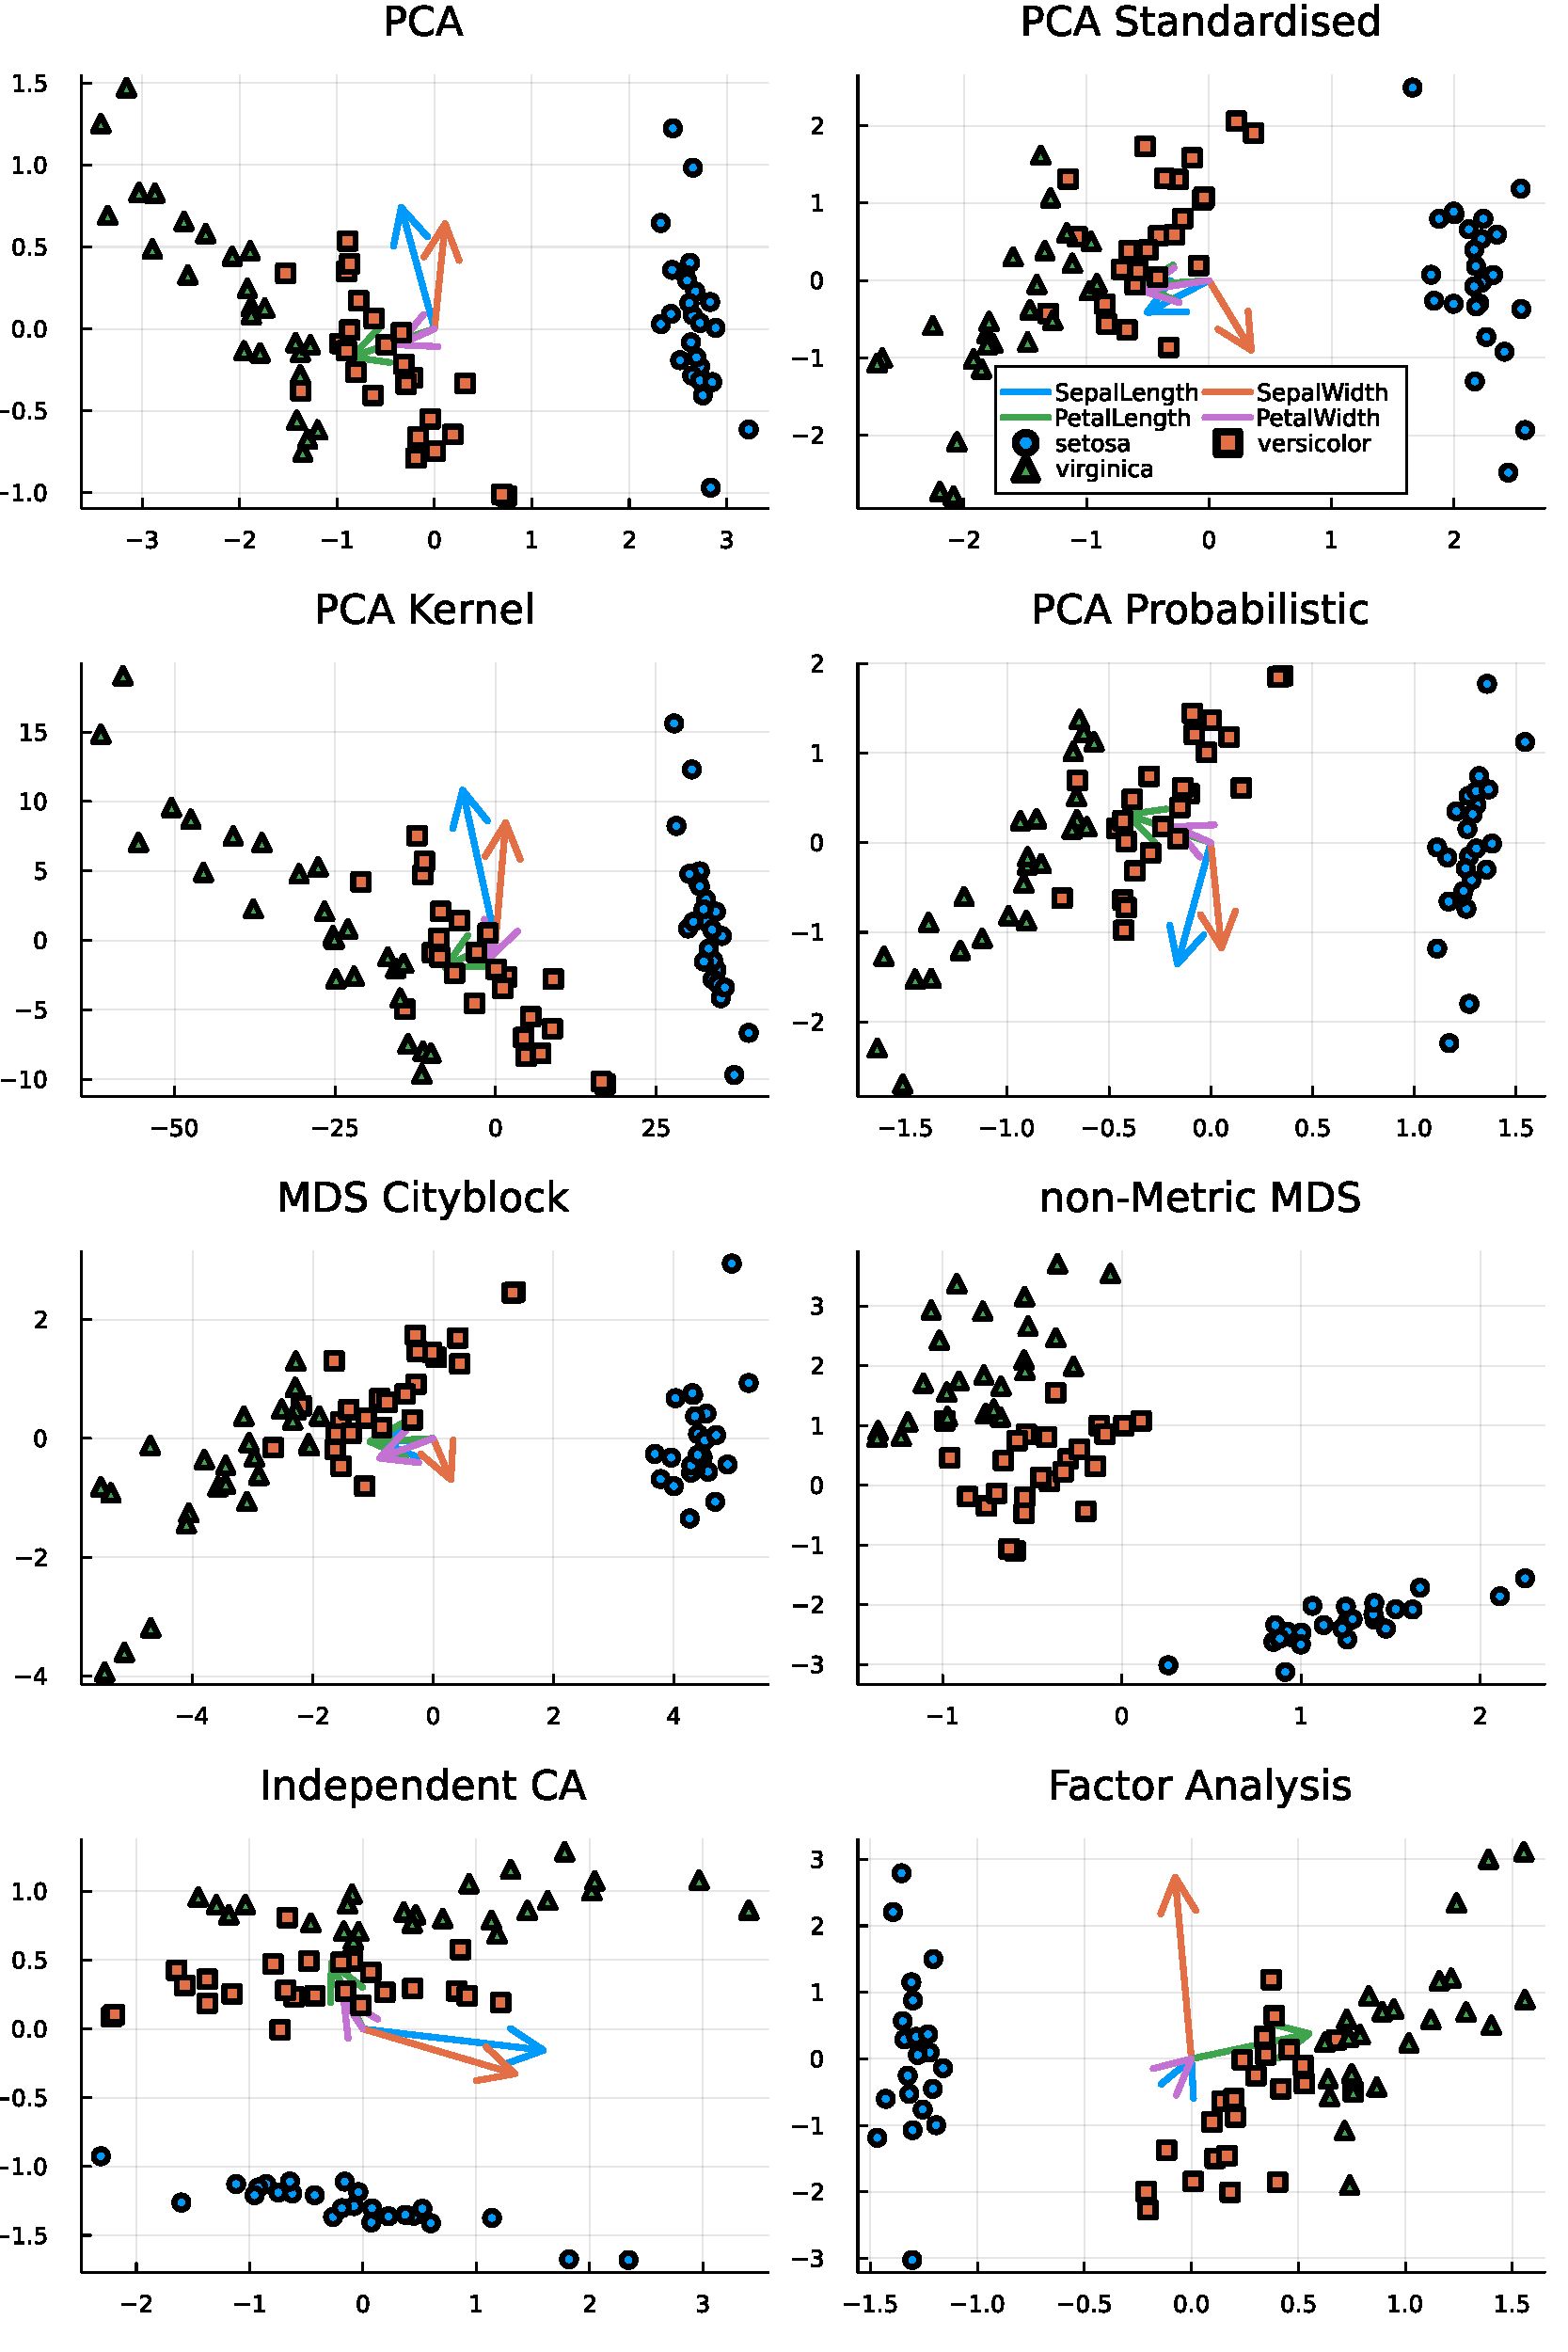
\includegraphics[width=.95\columnwidth]{pca.pdf}
\end{figure}

\subsection{Canonical Correlation Analysis -- Kanonische Korrelationsanalyse}

Findet für zwei Datensätze zwei Projektionen, um sie in einen gemeinsamen Raum
mit maximalen Korrelationen umzuwandeln.

\begin{lstlisting}
using MultivariateStats, RDatasets, Statistics
iris = dataset("datasets", "iris")
X = Matrix(iris[:,1:2])'  #; Sepal length, width
Y = Matrix(iris[:,3:4])'  #; Petal length, width
z = iris[:,5]             #; Art

round.(cor([X;Y], dims=2); digits=2)
 # 1.0   -0.12   0.87   0.82
 #-0.12   1.0   -0.43  -0.37
 # 0.87  -0.43   1.0    0.96
 # 0.82  -0.37   0.96   1.0

cca = fit(CCA, X, Y)
projection(cca, :y)
cor(cca)                  # 0.94 0.12
Xc = predict(cca, X, :x)
Yc = predict(cca, Y, :y)
round.(cor([Xc;Yc], dims=2); digits=2)
 # 1.0   0.0   0.94  0.0
 # 0.0   1.0   0.0   0.12
 # 0.94  0.0   1.0   0.0
 # 0.0   0.12  0.0   1.0

using Plots
shp = [:circle,:rect,:utriangle]
species = unique(z)
p = plot(layout=(1,2), size=(800,300))
for k=1:2, i=1:3
  j = z .== species[i]
  scatter!(p[k], Xc[k,j], Yc[k,j], label=species[i],
   markershape=shp[i], markercolor = i)
end
plot!(p[2], legend=false)
plot!(p[1], title="CCA - Dim=1")
plot!(p[2], title="CCA - Dim=2")
savefig("cca.pdf")
\end{lstlisting}

\begin{figure}[ht]
  \centering
  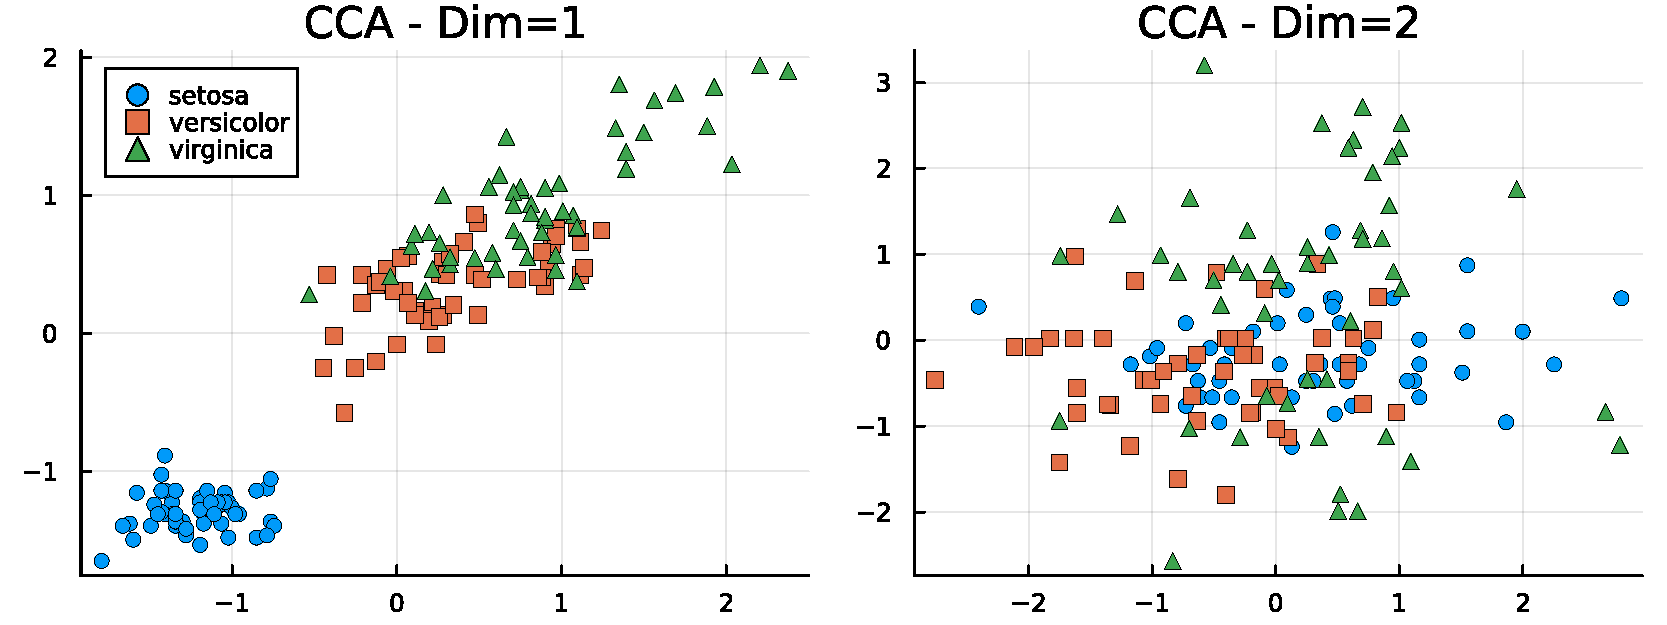
\includegraphics[width=.95\columnwidth]{cca.pdf}
\end{figure}

\section{Diskriminanzanalyse}

Mit \lstinline|MultivariateStats| Version: 0.10.2
(\href{https://juliastats.org/MultivariateStats.jl/stable/lda/}{doc}).

Unterscheiden von Gruppen die mit Merkmalen (Variablen) beschrieben werden.

Siehe auch
\hyperref[ssec:EntscheidungsbaumKlassifikation]{Entscheidungsbaum/Klassifikation}
und \hyperref[sec:NearestNeighbors]{NearestNeighbors}.

\begin{lstlisting}
using MultivariateStats, RDatasets, StatsBase, Distances
iris = dataset("datasets", "iris") #; Daten
# Kelchblatt-Sepal, Kronblatt-Petal, Länge/Breite
M = Matrix(iris[1:2:end,1:4])'     #; Trainingsdaten
s = iris[1:2:end,5]    # Art setosa virginica versicolor
Mt = Matrix(iris[2:2:end,1:4])'    #; Testdaten
st = iris[2:2:end,5]

# Lineare Diskriminanzanalyse für zwei Klassen
Mj = M[:,s .== "versicolor"]  #; Positive Klasse
Mn = M[:,s .!= "versicolor"]  #; Negative Klasse
stb= st .== "versicolor"      #; Testklassen true/false
lda = fit(LinearDiscriminant, Mj, Mn)  #; LDA schätzen
Mp = predict(lda, Mt)         #; true/false Schaetzung
countmap(Mp .== stb)
 # 0 => 19  1 => 56; 19 falsch 56 richtig
(MultivariateStats.evaluate(lda, Mt) .>= 0) == Mp  # true
(lda.b .+ sum(lda.w .* Mt, dims=1) .>= 0) == Mp'   # true

# Lineare Diskriminanzanalyse für merhrere Klassen
lda = fit(MulticlassLDA, M, s; outdim=2)  #; LDA schätzen
Mp = predict(lda, M)   #; Trainings Matrix transformieren
Mtp = predict(lda, Mt) #; Testmatrix
# Abstände^2 zu Klassenmittel
d = pairwise(SqMahalanobis(cov(Mp')), Mtp, lda.pmeans)
# Klassifizieren nach geringstem Abstand
k = unique(s)[getindex.(argmin(d, dims = 2), 2)]
countmap(k .== st)
 # 0 => 2, 1 => 73; 2 falsch 73 richtig
## Klassenwarscheinlichkeiten nach Distanzen
# Dazu gibt es unterschiedliche Varianten
x = exp.(-d./2)
# Modifiziren mit Apriori Wahrscheinlichkeit, Kosten, ...
x .*= (lda.stats.cweights ./ lda.stats.tweight)'
x ./= sum(x, dims=2)  #; Normieren damit Summe = 1
# Wahrscheinlichkeit nach Verteilung
using Distributions, LogarithmicNumbers
# Mittelwert und Kovarianz je Klasse aus
#  Beobachtungsdatensatz
msd = [[vec(mean(x; dims=2)), cov(x')] for S in
       unique(s) for x in [Mp[:,S .== s]]]
x = stack([logpdf(MvNormal(i[1], i[2]), Mtp)
           for i in msd])  #; Ln Klassenwarschinlichkeit
# Modifiziren mit Apriori Wahrscheinlichkeit, Kosten, ...
x .+= log.(lda.stats.cweights ./ lda.stats.tweight)'
x = exp.(ULogarithmic, x)
 #; Dieser Wert könnte verwendet werden für
 #; Wahrscheinlichkeit dass keine der Klassen zutrifft
x ./= sum(x, dims=2)       #; Normieren damit Summe = 1
# Klassifizieren nach größter Warscheinlichkeit
k = getindex.(argmax(x, dims = 2), 2)
unique(s)[k]               #; Klassennamen
countmap(unique(s)[k] .== st)
 # 0 => 2, 1 => 73; 2 falsch 73 richtig
b = stack([S .== st for S in unique(s)])  #; Binärmatrix
float(sum(x .* b, dims=1))   # 25.00 23.95 23.28; Richtig
float(sum(x .* .!b, dims=1)) #  0.00  1.72  1.05; Falsch

using Plots
shp = [:circle,:rect,:utriangle]
species = unique(s)
p = plot(layout=(1,2), size=(800,300))
proj = projection(lda)
for i=1:4
  plot!(p[2], [0,proj[i,1]], [0,proj[i,2]], arrow=true,
    label=names(iris)[i], linewidth=3)
end
for i in 1:3
  sp = species[i]
  j = st .== sp
  points = Mtp[:,j]
  scatter!(p[2], points[1,:], points[2,:], label=sp,
   markershape=shp[k[j]], color=[2,3,1][i])
end
scatter!(p[2], lda.pmeans[1,:], lda.pmeans[2,:],
 label="Klassenmittel", markershape=:star5, markersize=7)
plot!(p[2], legendfontsize=7, legend=:topleft)
plot!(p[2], title="LDA - Classification")

using Images
mima = extrema(Mp; dims=2)
xr = range(mima[2][1], mima[2][2], 100)
yr = range(mima[1][1], mima[1][2], 100)
x = [pdf(MvNormal(i[1], i[2]), [y, x]) for i in msd,
      x in xr,  y in yr]
x .*= lda.stats.cweights ./ lda.stats.tweight
x ./= maximum(x)
img = colorview(RGB, x .+ 1 .- maximum(x; dims=1))
plot!(p[1], vec(mima[1] .+ [-1 1]' .* yr.step.hi/2),
 vec(mima[2] .+ [-1 1]' .* xr.step.hi/2), img,
 yflip = false, aspect_ratio = :none)
for i in 1:3
  j = s .== species[i]
  scatter!(p[1], Mp[1,j], Mp[2,j], label=species[i],
   markershape=shp[i], color=[2,3,1][i])
end
plot!(p[1], title="LDA - Probapilities")
plot!(p[1], legendfontsize=8, legend=:bottom)
savefig("lda.pdf")
\end{lstlisting}

\begin{figure}[ht]
  \centering
  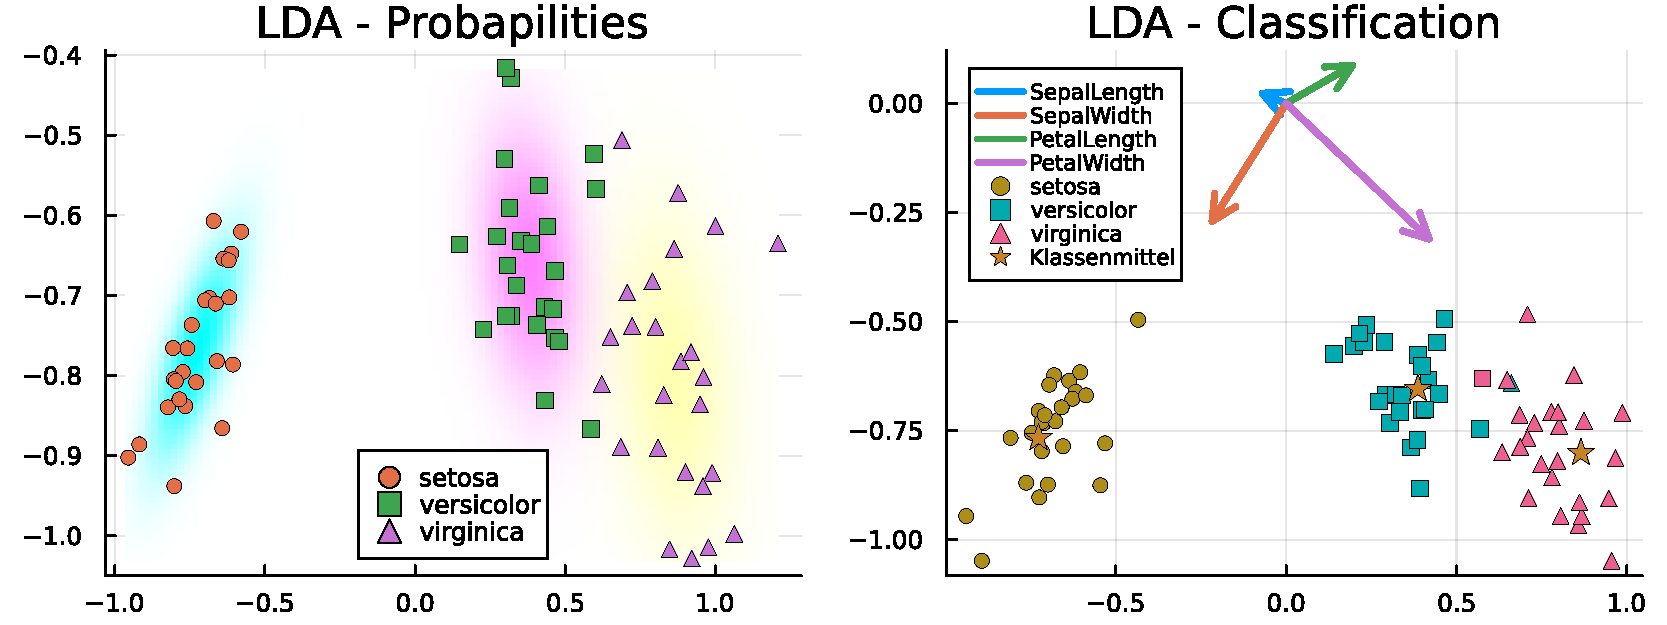
\includegraphics[width=.95\columnwidth]{lda.pdf}
\end{figure}

\section{Clustgering Clusteranalyse}

Version: 0.15.4
(\href{https://github.com/JuliaStats/Clustering.jl}{Git} /
\href{https://juliastats.org/Clustering.jl}{doc}).

\begin{lstlisting}
using RDatasets, Clustering, Plots, Distances, Random
Random.seed!(1)
iris = dataset("datasets", "iris"); # load the data
# Nur zwei Spalten verwenden
M = Matrix(iris[:, ["SepalWidth", "PetalWidth"]])'
s = iris.Species

rKmeans = kmeans(M, 3)  # K-means für 3 Cluster
rKmeans.centers         # Klassenmittel
 # 2.70755  3.45102   3.04167
 # 1.30943  0.244898  2.05208
# K-medoids
rKmedoids = kmedoids(pairwise(SqEuclidean(), M), 3)
# Hierarchical Clustering
rHclust = hclust(pairwise(SqEuclidean(), M);
 linkage=:single)  # Kleinste Distanz zu belibigem
rHclustB = hclust(pairwise(SqEuclidean(), M);
 linkage=:ward_presquared)  # min. dist^2 in Gruppen
# Markov Cluster Algorithm
rMcl = mcl(pairwise(SqEuclidean(), M))
# Affinity Propagation
rAffin = affinityprop(pairwise(SqEuclidean(), M))
# Density reachability
rDbscan = dbscan(M, .3, min_neighbors = 3,
 min_cluster_size = 20)
# Fuzzy C-means
rFuzzy = fuzzy_cmeans(M, 3, 2)

counts(rKmeans, rKmedoids)  # Kreuztabelle
 # 52   0   1
 #  0   0  49
 #  3  45   0
# Klassifizierungsähnlichkeit
randindex(rKmeans, rKmedoids)
 # (0.92, 0.96, 0.035, 0.93)
# Wie gut liegt jeder eilnzelne Punkt im Cluster
silhouettes(rKmeans, pairwise(Euclidean(), M))
# Variation of information
Clustering.varinfo(rKmeans, rKmedoids)  # 0.22
vmeasure(rKmeans, rKmedoids)            # 0.90
mutualinfo(rKmeans, rKmedoids)          # 0.90
# Confusion matrix
confusion(rKmeans, rKmedoids)
 # 3495   187
 #  205  7288

P = function(p, z, T="")
  shp = [:circle,:rect,:utriangle]
  scatter!(p, M[1,:], M[2,:], marker_z=z,
   markershape=shp[s.refs], title=T, color=:brg)
end
p = plot(layout=(4,2), size=(800,1200), legend=false)
P(p[1], rKmeans.assignments, "K-Means")
P(p[2], rKmedoids.assignments, "K-Medoids")
P(p[3], cutree(rHclust; k=3),
 "Hierarchical Clustering - Single")
P(p[4], cutree(rHclustB; k=3),
 "Hierarchical Clustering - Ward")
P(p[5], rMcl.assignments, "Markov Cluster Algorithm")
P(p[6], rAffin.assignments, "Affinity propagation")
P(p[7], rDbscan.assignments, "DBSCAN")
P(p[8], getindex.(argmax(rFuzzy.weights, dims = 2), 2),
 "Fuzzy C-means")
savefig("cluster.pdf")
\end{lstlisting}

\begin{figure}[ht]
  \centering
  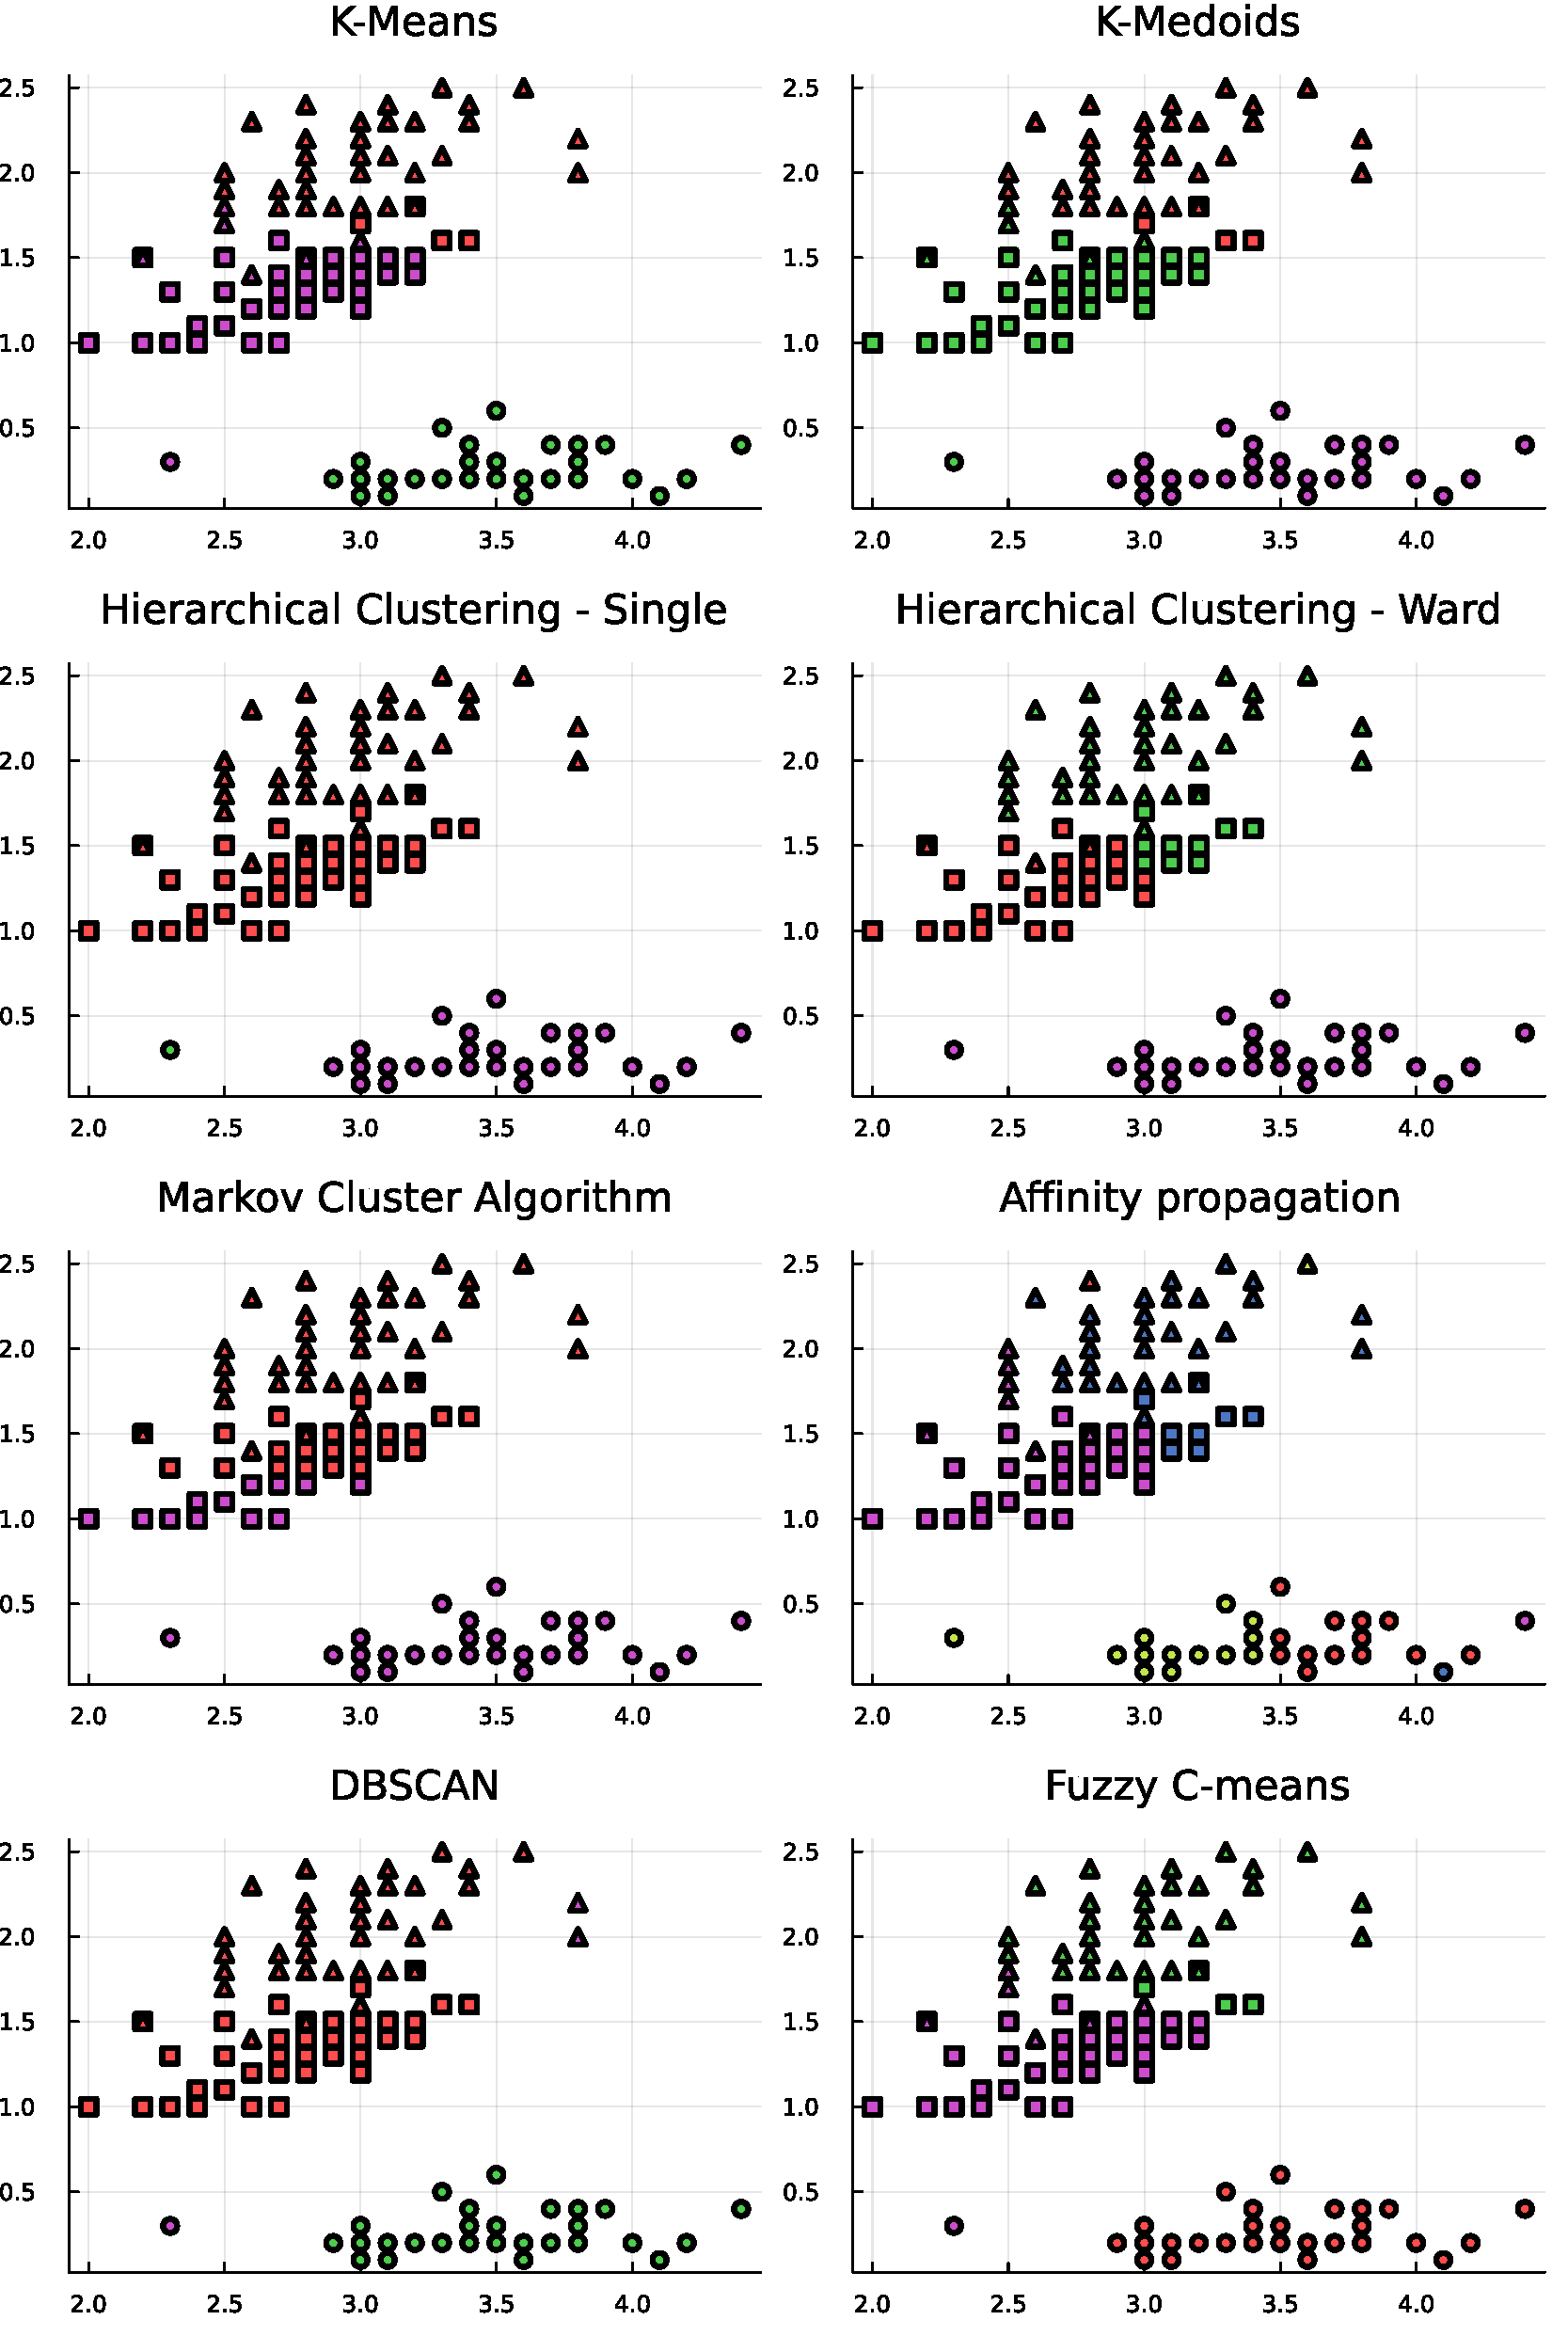
\includegraphics[width=.95\columnwidth]{cluster.pdf}
\end{figure}

\section{Regression}

\subsection{Base}

Koeffizienten von linearen Regressionen können ohne zusätzliche Pakete mit
\lstinline|\| geschätzt werden.

\begin{lstlisting}
X = [[1,1,1,1,1] [1,2,3,4,5]]
y = [2,4,7,10,9]
# y = c[1] * X[:,1] + c[2] * X[:,2]
c = X\y              # 0.4 2.0; Koeffizienten
# y = c[1] * X[:,1] + c[2] * X[:,2] + c[3] * X[:,2]^2
c = [X X[:,2].^2]\y  # -2.6 4.57 -0.43
\end{lstlisting}

\subsection{MultivariateStats}

Mit \lstinline|MultivariateStats| Version: 0.10.2
(\href{https://github.com/JuliaStats/MultivariateStats.jl}{Git} /
\href{https://juliastats.org/MultivariateStats.jl}{doc}) können lineare, ridge
und isotonic Regressionen erstellt werden.

\begin{lstlisting}
using MultivariateStats
X = [1,2,3,4,5]
y = [2,4,7,10,9]
llsq(X, y)         # 2 0.4; Slope Intercept
llsq([X X.^2], y)  # 4.57 -0.43 -2.6
ridge(X, y, 0.1)   # 1.98 0.46
isotonic(X, y)     # 2 4 7 9.5 9.5
\end{lstlisting}

\subsection{StatsModels -- Formula}

Erleichtert die Umwandlung von Daten in eine Matrix für Regressionen. Siehe
auch \hyperref[ssec:kategorialeVariablen]{Regression/GLM -- Kategoriale
Variablen} (\href{https://juliastats.org/StatsModels.jl/stable/formula/}{doc}).

\begin{lstlisting}
y ~ 1 + a + b + c + b&c

~ .. Formula Separator
1 .. Intercept (Automatisch), 0 .. kein Intercept
a, b, c .. Spalten a, b und C
 Falls Spalte nicht Numeric wird sie contrast coded/Dummy
& .. Interaction Term, Modellmatrix für jedes Spaltenpaar

b + c + b&c  ist Equivalent mit  b*c
(a + b) & c  ergibt  a & c  und  b & c

y ~ 1 + a + log(1+a) .. Intercept, Spalte a und log(1+a)
log(y) ~ 1 + a + b .. Transformation der Abhängigen
y ~ 1 + a + protect(1+a) .. Intercept, a und (1+a)

y ~ 1 + a + a&b   Ist Equvalent mit
Term(:y)~ConstantTerm(1) + Term(:a) + Term(:a) & Term(:b)

y ~ 1 + a + b   Ist Equvalent mit
term(:y) ~ foldl(+, term.((1, :a, "b")))
term(:y) ~ sum(term.((1, :a, "b")))
\end{lstlisting}

Mehrere Regressionen mit verschiedenen Spalten können mithilfe einer Schleife
realisiert werden.

\begin{lstlisting}
using DataFrames, GLM
df = DataFrame(reshape(1:40,:,4), ["y","x1","x2","x3"])
# Regression y~x1, y~x2 und y~x3
for x in names(df)[2:end]
  @show lm(term(:y) ~ term(x), df)
end
# Oder über Auswahl der Spalten
for i in 2:ncol(df)
  @show lm([ones(nrow(df)) df[:,i]], df.y)
end
\end{lstlisting}

\subsection{GLM}

Koeffizienten von linearen und verallgemeinerten linearen Modelle können mit
\lstinline|GLM| (Version 1.8.3.,
\href{https://github.com/JuliaStats/GLM.jl}{Git} /
\href{https://juliastats.org/GLM.jl/stable/}{doc}) geschätzt werden.

\subsubsection{Linear}

\begin{lstlisting}
using GLM
X = [[1,1,1,1,1] [1,2,3,4,5]]
y = [2,4,7,10,9]
ols = fit(LinearModel, X, y)     #; Lineare Regression
ols = lm(X, y)                   #; Alternative
using DataFrames
data = DataFrame(X=[1,2,3,4,5], y=[2,4,7,10,9])
ols = lm(@formula(y ~ X), data)  #; Alternative
coeftable(ols)           #; Koefizienten mit Signifikanz
ols                              #; Alternative
 #              Coef.  Std. Error     t  Pr(>|t|)
 # (Intercept)    0.4    1.38082   0.29    0.7909
 # X              2.0    0.416333  4.80    0.0172
  #  Lower 95%  Upper 95%
  #  -3.99439     4.79439
  #   0.675042    3.32496
coef(ols)          # 0.4 2.0; Koefizienten
coefnames(ols)     # (Intercept) X; Namen
deviance(ols)      # 5.2; Standardaweichung Modell
nulldeviance(ols)  # 45.2; Standardaweichung 0-Modell
# Modelschätzwerte
fitted(ols)        # 2.4 4.4 6.4 8.4 10.4
predict(ols)       #; Modelschätzwerte
predict(ols, DataFrame(X=[0,5]))
 # 0.4 10.4; Modelschätzwerte mit neuen Daten
response(ols)      # 2 4 7 10 9; Originalwerte
residuals(ols)     # -0.4 -0.4 0.6 1.6 -1.4; Residuen
cooksdistance(ols)
 # 0.17 0.03 0.03 0.45 2.12; Einfluss der Datenpunkte
r2(ols)            # 0.885; Korrelation
adjr2(ols)         # 0.847; Adjustierte Korrelation
confint(ols)       #; Konfidenzinterval der Koeffizienten
 # -3.99439   4.79439
 #  0.675042  3.32496
stderror(ols)      #; Standardfehler der Koeffizienten
 # 1.38 0.42
vcov(ols)  #; Varianz-Kovarianz-Matrix der Koeffizienten
 #  1.90667  -0.52
 # -0.52      0.173333
dof(ols)    # 3; Konsumierte Freiheitsgrade des Modells
nobs(ols)   # 5; Anzahl unabhängiger Beobachtungen
ftest(ols.model)  #; Unterschied Modell zu 0-Modell
 # 0.0172; Signifkikant
ols2 = lm(@formula(y ~ X + X^2), data)
ftest(ols.model, ols2.model)  #; Unterschied ols zu ols2
 # 0.30; Nicht signifikant
using StatsBase
aic(ols)   # 20.4; Akaike's Information Criterion
aicc(ols)  # 44.4; Corrected Akaike's for small samples
bic(ols)   # 19.2; Bayesian Information Criterion

using Plots
p = plot(layout=(1,2), size=(800,400))
scatter!(p[1], data.X, data.y, label="Beobachtung",
 xlabel="X", ylabel="y")
Plots.abline!(reverse(coef(ols))..., label="ols",
 linewidth=3)
ND = DataFrame(X=1:.25:5)  # Neue Daten
plot!(p[1], ND.X, predict(ols2, ND), label="ols2",
 linewidth=3)
scatter!(p[2], fitted(ols), residuals(ols), label="ols",
 xlabel="Predicted", ylabel="Residuen", color=2)
scatter!(p[2], fitted(ols),residuals(ols2),label="ols2",
 color=3)
savefig("glm.pdf")
\end{lstlisting}

\begin{figure}[ht]
  \centering
  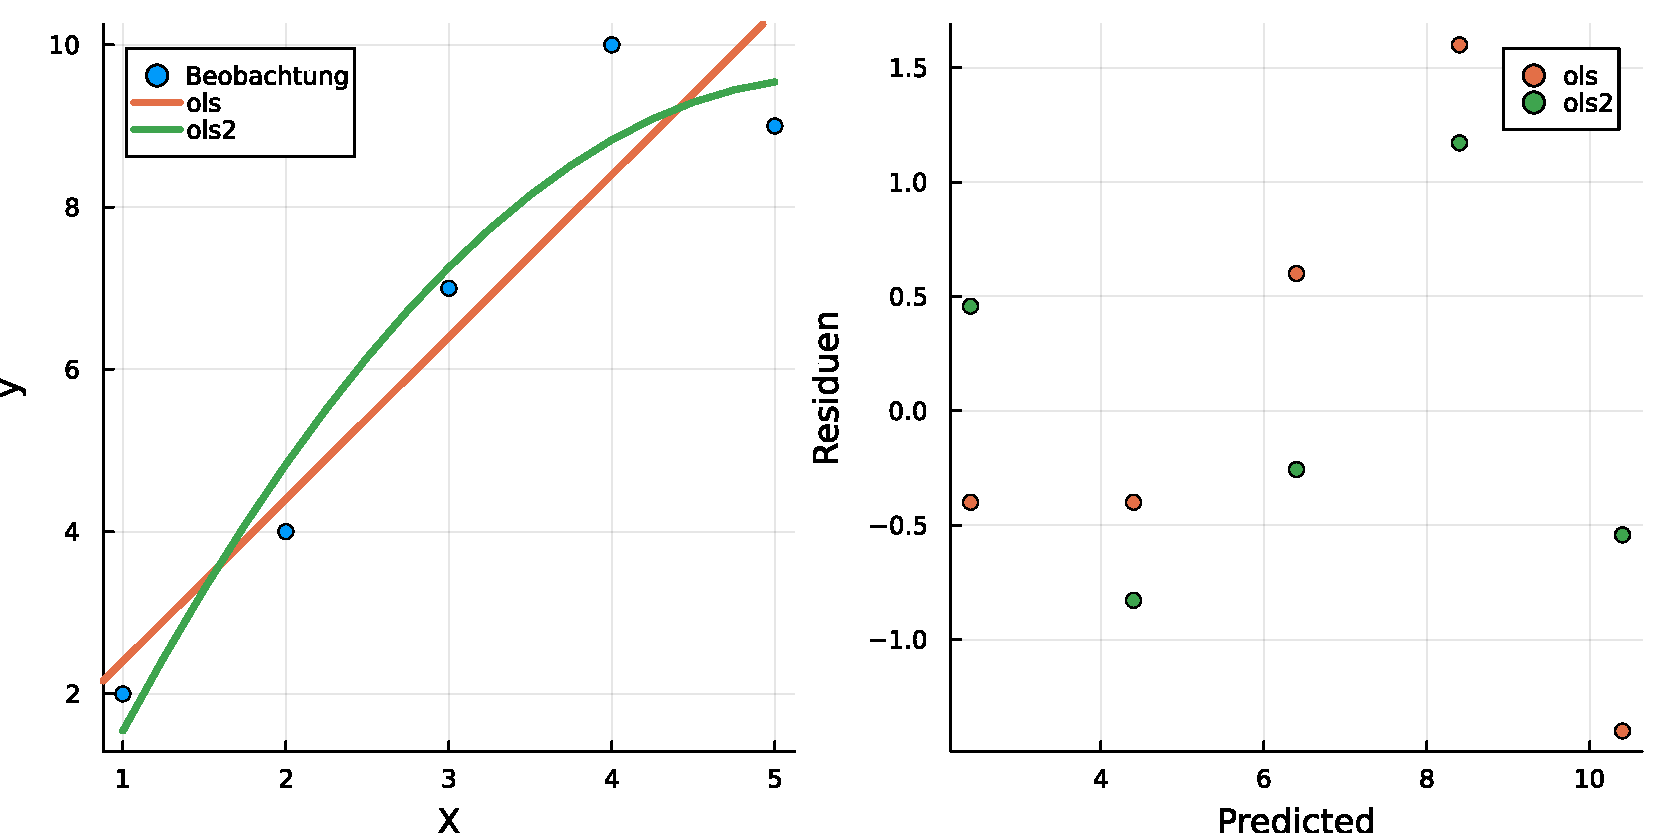
\includegraphics[width=.95\columnwidth]{glm.pdf}
\end{figure}

\subsubsection{Kategoriale Variablen}
\label{ssec:kategorialeVariablen}

Diese werden automatisch als Dummy--Matrix codiert.

\begin{lstlisting}
using GLM, DataFrames
data = DataFrame(X=[1,2,3,4,5], c=["a","a","b","b","b"],
 y=[2,4,7,10,13])
# Intercept und Differenz dazu
ols = lm(@formula(y ~ c), data)
 # (Intercept)    3.0
 # c: b           7.0
# Intercept je Gruppe
ols = lm(@formula(y ~ 0 + c), data)
 # c: a    3.0
 # c: b   10.0
# Intercept Differenz, gemeinsamer Anstieg
ols = lm(@formula(y ~ c + X), data)
 # (Intercept)  -1.2
 # c: b          0.0
 # X             2.8
# Intercept, Anstieg und Differenz dazu
ols = lm(@formula(y ~ c * X), data)
 # (Intercept)   0.0
 # c: b         -2.0
 # X             2.0
 # c: b & X      1.0
# kein Inercept, Anstieg je Gruppe
ols = lm(@formula(y ~ 0 + c & X), data)
 #c: a & X   2.0
 #c: b & X   2.52
# Gemeinsames Intercept; Anstieg je Gruppe
ols = lm(@formula(y ~ c & X), data)
 # (Intercept)  -0.75
 # c: a & X      2.45
 # c: b & X      2.7
# Intercept Differenz, Anstieg je Gruppe
ols = lm(@formula(y ~ c + c & X), data)
 # (Intercept)   0.0
 # c: b         -2.0
 # c: a & X      2.0
 # c: b & X      3.0
# Intercept und Anstieg je Gruppe
ols = lm(@formula(y ~ 0 + c + c & X), data)
 # c: a        0.0
 # c: b       -2.0
 # c: a & X    2.0
 # c: b & X    3.0
\end{lstlisting}

\subsubsection{Generalized Linear}

Für eine GLM muss deren Verteilung (\lstinline|family|) und Funktion
(\lstinline|link|) angegeben werden. Mit \lstinline|?Link| kann man alle
verfügbaren Linktypen anzeigen.

\begin{lstlisting}
using GLM, DataFrames

## Binomial Logit Modell
data = DataFrame(X=[1,2,2,3], y=[0,0,1,1])
logit = glm(@formula(y ~ X), data,Binomial(),LogitLink())
logit = glm(@formula(y ~ X), data, Binomial())  #; Gleich
1 ./ (1 .+ exp.(-coef(logit)[1].-coef(logit)[2].*data.X))
predict(logit)                                  #; Gleich
# Werte zwischen 0 und 1
data = DataFrame(X=[1,2,3], y=[0,0.5,1])
logit = glm(@formula(y ~ X), data, Binomial())

## Poisson Log Modell
data = DataFrame(X=[1,2,3,4], y=[2,6,4,50])
reg = glm(@formula(y ~ X), data, Poisson(), LogLink())
reg = glm(@formula(y ~ X), data, Poisson())     #; Gleich
exp.(coef(reg)[1] .+ coef(reg)[2] .* data.X)
predict(reg)                                    #; Gleich
# Mit anderen Verteilungen
r2 = glm(@formula(y ~ X), data, Gamma(), LogLink())
r3 = glm(@formula(y~X),data,InverseGaussian(),LogLink())
r4 = glm(@formula(y ~ X), data, Normal(), LogLink())
r5 = lm(@formula(log(y) ~ X), data)

using Plots
ND = DataFrame(X=1:0.2:4)
p = plot(layout=(1,2), size=(800,300))
plot!(p[1], ND.X, predict(reg, ND), linewidth=3,
 label="Poisson")
plot!(p[1], ND.X, predict(r2, ND), linewidth=3,
 label="Gamma")
plot!(p[1],ND.X,predict(r3,ND), linewidth=3,
 label="InverseGaussian")
plot!(p[1], ND.X, predict(r4, ND), linewidth=3,
 label="Normal")
plot!(p[1], ND.X, exp.(predict(r5,ND)),
 linewidth=3, label="Linearisiert")
scatter!(p[1], data.X, data.y, label="Beobachtung")

scatter!(p[2], data.X, data.y - predict(reg),
 label="Poisson", legend=:topleft, ylabel="Residuen")
scatter!(p[2], data.X, data.y-predict(r2), label="Gamma")
scatter!(p[2], data.X, data.y - predict(r3),
 label="InverseGaussian")
scatter!(p[2], data.X, data.y-predict(r4),label="Normal")
scatter!(p[2], data.X, data.y - exp.(predict(r5)),
 label="Linearisiert")
savefig("glmLogLink.pdf")

D1 = DataFrame(X=[1,2,3], y=[0  ,3,7])
D2 = DataFrame(X=[1,2,3], y=[0.1,3,7])
glm(@formula(y ~ X), D1, Poisson(), LogLink())  #; OK
# glm(@formula(y ~ X), D2, Poisson(), LogLink())
 #; Error wegen 0.1
# glm(@formula(y ~ X), D1, Normal(), LogLink())
 #; Error wegen 0
glm(@formula(y ~ X), D2, Normal(), LogLink())   #; OK
\end{lstlisting}

\begin{figure}[ht]
  \centering
  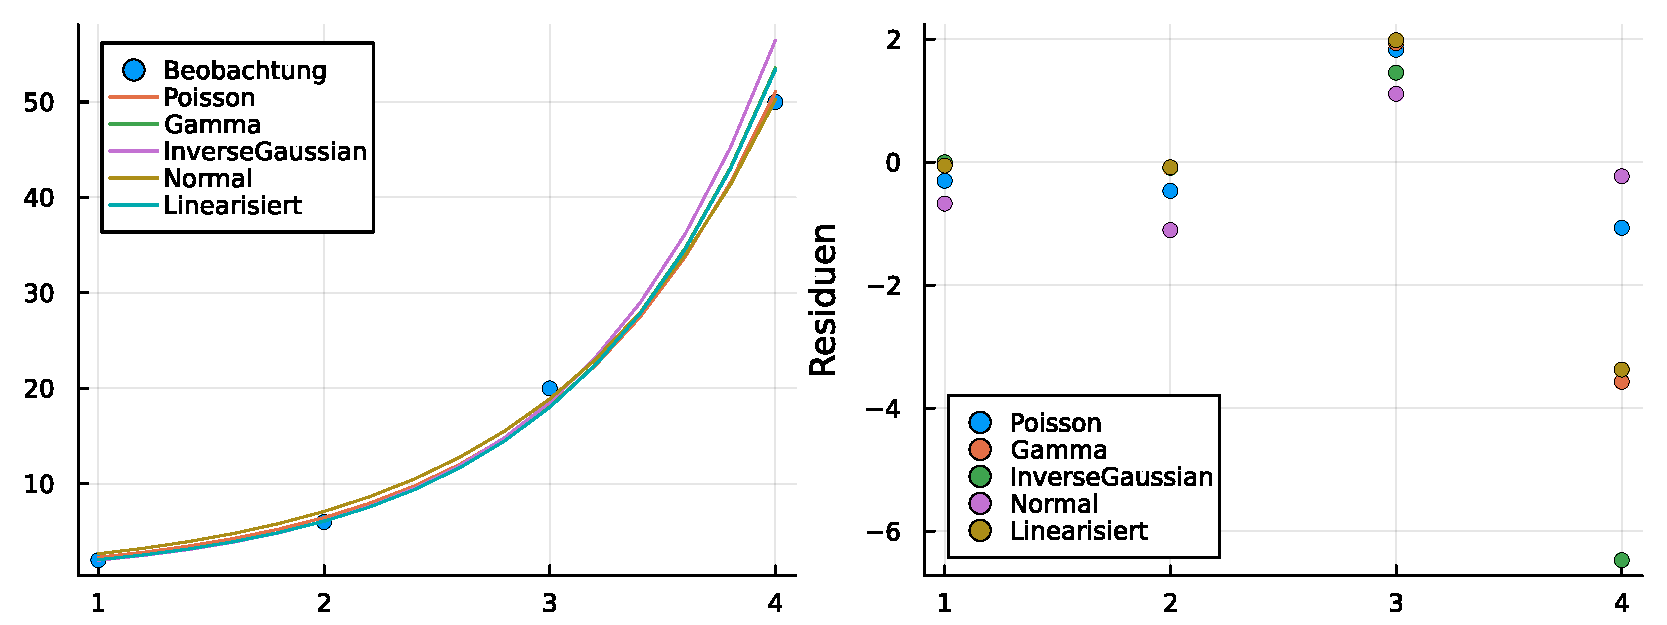
\includegraphics[width=.95\columnwidth]{glmLogLink.pdf}
\end{figure}

\subsection{Lasso}

Lasso \lstinline|v0.7.0| (Least absolute shrinkage and selection operator --
kleinster absoluter Reduzierungs-- und Auswahloperator) kann bei der
Variablenauswahl und Regularisierung helfen, um die Vorhersagegenauigkeit und
Interpretierbarkeit zu verbessern
(\href{https://github.com/JuliaStats/Lasso.jl}{Git} /
\href{https://juliastats.org/Lasso.jl/stable/}{doc}).


\begin{lstlisting}
using Lasso, DataFrames, RDatasets
iris = dataset("datasets", "iris")

# Lasso für GLM mit Family=Normal, Link=LogLink
# ridge (α=0), lasso (α=1)
# Für α=0 muss λ angegeben werden
path = fit(LassoPath,
 @formula(SepalLength ~ PetalLength + log(PetalLength) +
                        PetalLength^2 + 1/PetalLength),
 iris, Normal(), LogLink(); α=0.5)
coef(path, AllSeg())  # Koeffizienten des gesamten Pfades
# Koeffizienten wo AICc minimal
coef(path, MinAICc())  # [1] 1.59 [4] 0.0099
coef(path, MinAIC())   # min AIC
coef(path, MinBIC())   # min BIC
# Cross-validation
# nCVfolds=10 Datensatz in 10 zufällige Teile teilen
coef(path, MinCVmse(path, 10))  # minimum mse
coef(path, MinCV1se(path, 10))  # largest λt
# Detailierte Koeffizientenangabe
selectmodel(path.model, MinAICc())
 #          Coef.  Std. Error     z  Pr(>|z|)
 # x1  1.58654       3.75845   0.42    0.6729
 # x2  0.0           2.68277   0.00    1.0000
 # x3  0.0           7.57216   0.00    1.0000
 # x4  0.00993123    0.140455  0.07    0.9436
 # x5  0.0           6.34331   0.00    1.0000
  #  Lower 95%  Upper 95%
  #  -5.77989    8.95298
  #  -5.25813    5.25813
  # -14.8412    14.8412
   #  -0.265355   0.285217
 # -12.4327    12.4327

# Selektiert ein Modell
using Random, MLBase  #; Für Kfold in MinCVmse
m = fit(LassoModel,
 @formula(SepalLength ~ PetalLength + log(PetalLength) +
                        PetalLength^2 + 1/PetalLength),
 iris, Normal(), LogLink();
 select=MinCVmse(Kfold(nrow(iris), 10)))

# Als Ausreichend ausgewählt
m = fit(LassoModel,
 @formula(SepalLength ~ PetalLength^2),
 iris, Normal(), LogLink(); select=MinAIC())
coef(m)                         # 1.59 0.00993
# GLM zum Vergleich
glm = fit(GeneralizedLinearModel,
 @formula(SepalLength ~ PetalLength^2),
 iris, Normal(), LogLink())
coef(glm)                       # 1.59 0.0100
std(predict(m) - predict(glm))  # 0.00525
\end{lstlisting}

\subsection{MixedModels}

Gemischte Modelle (\lstinline|v4.22.1|
\href{https://github.com/JuliaStats/MixedModels.jl}{Git} /
\href{https://juliastats.org/MixedModels.jl/stable/}{doc}) differenzieren
zwischen festen und zufälligen Effekten.

\subsubsection{Scalar random effects}

Skalare Zufallseffekte, als Verschiebung des Intercepts je Gruppe
\lstinline|G|, werden mit \lstinline"(1|G)" in \lstinline|@formula|
angegeben.

\begin{lstlisting}
using MixedModels
dyestuff = MixedModels.dataset(:dyestuff)  #; Daten
# Zufallsefekt von batch mit Intercept bereücksichtigen
fm = @formula(yield ~ (1|batch)) #; Intercept automatisch
fm = @formula(yield ~ 1 + (1|batch)) #; Gleich
fm1 = fit(MixedModel, fm, dyestuff) #; maximum likelihood
# REML - Restricted maximum likelihood
fm1reml = fit(MixedModel, fm, dyestuff, REML=true)

fm1.beta              # 1527.5; Fixe Effekte
coef(fm1)             #; Das Gleiche
fixef(fm1)            #; Das Gleiche
coeftable(fm1)        #; Als Tabelle
 #               Coef.  Std. Error      z  Pr(>|z|)
 # (Intercept)  1527.5     17.6946  86.33    <1e-99

fm1.b                 #; Zufallsefekte
 # -16.63  0.37  26.97  -21.8  53.58  -42.49
ranef(fm1)            #; Das Gleiche
only(raneftables(fm1))  #; Als Tabelle

# Zum Vergleich Mittel und Median
using DataFrames, Statistics, GLM
d = DataFrame(dyestuff)
m = mean(d.yield)     # 1527.5
LM = lm(@formula(yield ~ 0 + batch), d)
md = median(d.yield)  # 1530.0
gd = combine(groupby(d, :batch), :yield => median)
["Modell\batch" "fix" permutedims(unique(dyestuff.batch))
"MMMaxLi" fm1.beta round.(ranef(fm1)[1]; digits=1)
"MMReml" fm1reml.beta round.(ranef(fm1reml)[1]; digits=1)
"lm mean" m (coef(LM) .- m)'
"median" md (gd[:,2] .- md)']
 # "Modell\batch"      "fix"     "A"    "B"    "C"
 # "MMMaxLi"       1527.5     -16.6    0.4   27.0
 # "MMReml"        1527.5     -17.6    0.4   28.6
 # "lm mean"       1527.5     -22.5    0.5   36.5
 # "median"        1530.0     -10.0   10.0   30.0
  #    "D"    "E"     "F"
  # -21.8   53.6   -42.5
  # -23.1   56.7   -45.0
  # -29.5   72.5   -57.5
  # -65.0   95.0   -75.0
\end{lstlisting}

Mehrere Gruppen werden mit \lstinline|+| verbunden: \lstinline"(1|G) + (1|H)".

\begin{lstlisting}
using MixedModels
penicillin = MixedModels.dataset(:penicillin)
fm3 = fit(MixedModel, @formula(diameter ~ 1 + (1|plate) +
    (1|sample)), penicillin)
fixef(fm3)  # 22.97
raneftables(fm3)[1]
 #     plate  (Intercept)
 # 1 | a      0.804403
 # 2 | b      0.804403
 # : | :         :
raneftables(fm3)[2]
 #     sample  (Intercept)
 # 1 | A       2.18566
 # 2 | B       -1.00983
 # : | :         :
\end{lstlisting}

Bei hierarchischer (nested) Gruppierung wird \lstinline|/| verwendet:
\lstinline"(1|G/H)", wobei \lstinline|H| Untergruppen sind, die in \lstinline|G|
enthalten sind. Wenn die Bezeichnungen (levels) der inneren Gruppe
ausschließlich (unique) in der ihr übergeordneten Gruppe zu finden sind, muss
diese Verschachtelung nicht explizit in der Modellsyntax ausgedrückt werden und
kann dann auch mit \lstinline"(1|G) + (1|H)" beschrieben werden.

\begin{lstlisting}
using MixedModels, DataFrames
pastes = DataFrame(MixedModels.dataset(:pastes))
fm4a = fit(MixedModel, @formula(strength ~ 1 +
 (1|batch/cask)), pastes)
pastes.sample = (string.(pastes.batch, "&", pastes.cask))
fm4b = fit(MixedModel, @formula(strength ~ 1 +
 (1|sample) + (1|batch)), pastes)
fixef(fm4a)  # 60.05
fixef(fm4b)  # 60.05
raneftables(fm4a)[1]
 #     batch & cask  (Intercept)
 # 1 | ("A", "a")    1.92557
 # 2 | ("A", "b")    0.483539
 # : |      :         :
raneftables(fm4b)[1]
 #    sample  (Intercept)
 # 1 | A&a     1.92557
 # 2 | A&b     0.483539
 # : |      :         :
raneftables(fm4a)[2]
 #     batch  (Intercept)
 # 1 | A      0.643691
 # 2 | B      -0.219088
 # : |      :         :
raneftables(fm4b)[2]
 #     batch  (Intercept)
 # 1 | A      0.643691
 # 2 | B      -0.219088
 # : |      :         :
\end{lstlisting}

\subsubsection{Vector--valued random effects}

Vektorwert Zufallseffekte, als Veränderung des Anstiegs von \lstinline|X| je
Gruppe \lstinline|G|, werden mit \lstinline"(X|G)" in \lstinline|@formula|
angegeben. Mit \lstinline"(1 + X|G)" wird sowohl Intercept als auch Anstieg je
Gruppe angepasst. Wobei hier auch die Korrelation zwischen den Zufallseffekten
für verschiedene Prädiktoren bestimmt wird. Diese Korrelation wird nicht
bestimmt (z.\,B.\ gewünscht, wenn viele Zufallseffekte vorhanden sind) wenn
\lstinline"(1|G) + (X|G)" oder \lstinline"zerocorr(1 + days|subj)" verwendet
wird.

\begin{lstlisting}
using MixedModels
sleepstudy = MixedModels.dataset(:sleepstudy)
fm2 = fit(MixedModel, @formula(reaction ~ 1 + days +
 (1 + days|subj)), sleepstudy)
VarCorr(fm2)
 # Variance components:
 #             Column    Variance Std.Dev.   Corr.
 # subj     (Intercept)  565.51068 23.78047
 #          days          32.68212  5.71683 +0.08
 # Residual              654.94145 25.59182
coeftable(fm2)
 #                 Coef.  Std. Error      z  Pr(>|z|)
 # (Intercept)  251.405      6.63226  37.91    <1e-99
 # days          10.4673     1.50224   6.97    <1e-11
only(raneftables(fm2))
 #     subj  (Intercept)  days
 # 1 | S308    2.81582     9.07551
 # 2 | S309  -40.0484     -8.64408
 # 3 | S310  -38.4331     -5.5134
 # : |  :         :           :

fm2b = fit(MixedModel, @formula(reaction ~ 1 + days +
 (1|subj) + (days|subj)), sleepstudy)
VarCorr(fm2b)
 # Variance components:
 #             Column    Variance Std.Dev.   Corr.
 # subj     (Intercept)  584.25897 24.17145
 #          days          33.63281  5.79938   .
 # Residual              653.11578 25.55613
coeftable(fm2b)
 #                 Coef.  Std. Error      z  Pr(>|z|)
 # (Intercept)  251.405      6.70771  37.48    <1e-99
 # days          10.4673     1.51931   6.89    <1e-11
only(raneftables(fm2b))
 #     subj  (Intercept)  days
 # 1 | S308  1.85472      9.23642
 # 2 | S309  -40.0225     -8.61744
 # 3 | S310  -38.7233     -5.43435
 # : |  :         :           :
\end{lstlisting}

Bei qualitativen Prediktoren werden Korrelationen zwischen allen Ausprägungen
(Levels) geschätzt. Mit \lstinline|zerocorr| und \lstinline|fulldummy| kann dies
verhindert werden.

\begin{lstlisting}
using MixedModels
sleepstudy = MixedModels.dataset(:sleepstudy)

# Korrelation zwischen jedem Level und auch Intercept
fm2c = fit(MixedModel, @formula(reaction ~ 1 + days +
 (1 + days|subj)), sleepstudy,
    contrasts = Dict(:days => DummyCoding()))
VarCorr(fm2c)
 # Variance components:
 #             Column    Variance  Std.Dev.   Corr.
 # subj     (Intercept)   955.69001 30.91424
 #          days: 1       493.28331 22.20998 -0.30
 #          days: 2       911.69517 30.19429 -0.57 +0.75
 #             :              :        :
coeftable(fm2c)
 # (Intercept)  256.652       7.36615  34.84    <1e-99
 # days: 1        7.84395     5.45319   1.44    0.1503
 # days: 2        8.71009     7.2789    1.20    0.2315
 #    :            :           :         :       :
only(raneftables(fm2c))
 #     subj  (Intercept)  days: 1   days: 2   days: 3 ...
 # 1 | S308  -7.72997     3.81182   -7.1743   46.5738 ...
 # 2 | S309  -34.3748     -24.2256  -27.2167  -43.7698...
 #   :   :   :

# Keine Korrelation
fm2d = fit(MixedModel, @formula(reaction ~ 1 + days +
 zerocorr(1 + fulldummy(days)|subj)), sleepstudy,
    contrasts = Dict(:days => DummyCoding()))
VarCorr(fm2d)
 # Variance components:
 #             Column     Variance    Std.Dev.    Corr.
 # subj     (Intercept)  1135.1084091 33.6913700
 #          days: 0       775.8089921 27.8533480   .
 #          days: 1       357.6378321 18.9113149   . .
 #          days: 2       221.0775456 14.8686767   . . .
 #             :              :        :
coeftable(fm2d)
 #                  Coef.  Std. Error      z  Pr(>|z|)
 # (Intercept)  256.652      10.7804   23.81    <1e-99
 # days: 1        7.84395     9.11488   0.86    0.3895
 # days: 2        8.71009     8.68874   1.00    0.3161
 #    :            :           :         :       :
only(raneftables(fm2d))
 #     subj  (Intercept)  days: 0   days: 1   days: 2 ...
 # 1 | S308  35.4252      -34.4738  -27.366   -27.4841...
 # 2 | S309  -73.5839     32.1622   9.53044   6.15799 ...
 #   :   :   :
\end{lstlisting}

Für eine GLMM muss deren Verteilung (\lstinline|family|) und bei Bedarf die
Funktion (\lstinline|link|) angegeben werden. Mit \lstinline|fast=true|, kann
eine schnellere, aber etwas ungenauere Anpassung erfolgen.

\begin{lstlisting}
using MixedModels
verbagg = MixedModels.dataset(:verbagg)
gm = fit(MixedModel, @formula(r2 ~ 1 + anger + (1|subj)),
         verbagg, Bernoulli(), LogitLink())
gm2 =fit(MixedModel, @formula(r2 ~ 1 + anger + (1|subj)),
          verbagg, Bernoulli(), LogitLink(), fast=true)
coeftable(gm)
 #                   Coef.  Std. Error      z  Pr(>|z|)
 # (Intercept)  -1.03138     0.278759   -3.70    0.0002
 # anger         0.0458044   0.0135466   3.38    0.0007
coeftable(gm2)
 #                   Coef.  Std. Error      z  Pr(>|z|)
 # (Intercept)  -0.984366    0.278734   -3.53    0.0004
 # anger         0.0436995   0.0135454   3.23    0.0013
\end{lstlisting}

\subsection{Quantille}

Qantillen Regression (\lstinline|v0.1.11|,
\href{https://github.com/pkofod/QuantileRegressions.jl}{Git})

\begin{lstlisting}
using QuantileRegressions, DataFrames, RDatasets
iris = dataset("datasets", "iris")

# Modell für 0.5 Quantille
m = qreg(@formula(SepalLength ~ PetalLength), iris, .5)
m
 #              Quantile  Estimate  Std.Error  t value
 # (Intercept)       0.5  4.35556   0.110287   39.4931
 # PetalLength       0.5  0.388889  0.0265785  14.6317
\end{lstlisting}

\subsection{Nichtlinear}

Nichtlineare Regressionen können z.\,B.\ mit \lstinline|LsqFit|
(\lstinline|v0.15.0|, \href{https://github.com/JuliaNLSolvers/LsqFit.jl}{Git} /
\href{https://julianlsolvers.github.io/LsqFit.jl/latest/}{doc}) geschätzt
werden.

\begin{lstlisting}
using LsqFit
# Modell bei dem Koeffizienten geschätz werden
@. model(X, p) = p[1]*exp(-X*p[2])
X = 0:5  # Unabhängige
y = [10,6,4,2,1,.5]      #; Abhängige
p0 = [1., 1.]            #; Startwerte
fit = curve_fit(model, X, y, p0)  #; Koeffizienten suchen
# Maximale Interationen, Schritte ausgeben (trace)
fit = curve_fit(model, X, y, p0; maxIter=99,
 show_trace=true)
coef(fit)                # 10.1 0.519; Schätzwerte
dof(fit)                 # 4; Freiheitsgrade
stderror(fit)            # 0.275 0.0264; Standardfehler
margin_error(fit, 0.05)  # 0.763 0.0733; Schwankugsbreite
confidence_interval(fit, 0.05)  #; Konfidenzinterval
 # (9.31, 10.8)
 # (0.446, 0.592)
fit.resid  #; Residuen
model(X, coef(fit))      #; Modelschätzwerte

lb = [1.0, 0.0]          #; Unter Grenze
ub = [5.0, Inf]          #; Obere Grenze
p0 = [2.5, 1.]           #; Startwerte
fitB = curve_fit(model, X, y, p0, lower=lb, upper=ub)
coef(fitB)               # 5.0 0.256; Schätzwerte

#Multivariat
X = [0:7 [1,3,6,9,15,24,42,63]]
y = [1,2,3,6,9,14,20,26]
function model(X, p)
  a, b, c, d, e = p      #; Paramternamen
  x = X[:,1]             #; Unabhängige x
  y = X[:,2]             #; Unabhängige y
  @. a + b*x^c + d*y^e
end
p0 = [1,.5,2,.1,.5]      #; Startwerte
fit = curve_fit(model, X, y, p0)  #; Koeffizienten suchen
\end{lstlisting}

\subsection{Entscheidungsbaum}

Siehe \hyperref[ssec:EntscheidungsbaumRegression]{Entscheidungsbaum/Regression}.

\section{Entscheidungsbaum}

Mit \lstinline|DecisionTree| (\lstinline|v0.12.3|,
\href{https://github.com/JuliaAI/DecisionTree.jl}{Git} /
\href{https://docs.juliahub.com/DecisionTree/pEDeB/0.12.3/}{doc}) können
Entscheidungsbäume zur Klassifikation oder Regression erstellt werden.

\subsection{Klassifikation}
\label{ssec:EntscheidungsbaumKlassifikation}

\begin{lstlisting}
using DecisionTree
X, y = load_data("iris")
# Für bessere Performance als konkrete Typen
X = float.(X)
y = string.(y)
s = ["sepal length","sepal width", "petal length",
 "petal width"]

# Entscheidungsbaum
model = build_tree(y, X,  #; labels, features
 0,   #; n rand gewählte Features (Def.: 0,alle behalten)
 -1,  #; maximale Baumtiefe (Def.: -1, kein Maximum)
 4,   #; Mindestanzahl auf Blatt (Def.: 1)
 8,   #; Mindestanzahl für Aufteilung (Def.: 2)
 .0;  #; Mindestreinheit, nach Aufteilung (Def.: 0.0)
 rng = 0)  #; Seed Zufallszahl
# Vereine Blätter
# die danach zu >=90% einer Klasse angehören
model = prune_tree(model, 0.9)
print_tree(model; feature_names=s)  #; Anzeigen
 # Feature 4: "petal width" < 0.8 ?
 # ├─ Iris-setosa : 50/50
 # └─ Feature 4: "petal width" < 1.75 ?
 #     ├─ Iris-versicolor : 49/54
 #     └─ Iris-virginica : 45/46
apply_tree(model, [5.9,3.0,5.1,1.9])  #; Anwenden
 # "Iris-virginica"
# Wahrscheinlichkeiten für Klassen
apply_tree_proba(model, [5.9,3.0,5.1,1.9], unique(y))
 # 0.0 0.02 0.98
preds = apply_tree(model, X)  #; Klassifizierung
# Confusion Matrix
DecisionTree.confusion_matrix(y, preds)
 # Accuracy: 0.96
 # Kappa:    0.94
 # 3×3 Matrix{Int64}:
 #  50   0   0
 #   0  49   1
 #   0   5  45
DecisionTree.accuracy(y, preds)  # 0.96; Treffer
# Einflussstärke der Daten
impurity_importance(model)  # 0 0 0 0.96
model.featim  #; Das Gleiche
split_importance(model)  # 0 0 0 2
p = permutation_importance(model, y, X, (model, y, X) ->
 DecisionTree.accuracy(y, apply_tree(model, X)),
 3; rng=42)
p.mean  # 0 0 0 0.67
p.scores  #; Für jeden der 3 Zufallsläufe
 # 0.0   0.0       0.0
 # 0.0   0.0       0.0
 # 0.0   0.0       0.0
 # 0.72  0.606667  0.693333
# Kreuzvalidierung (folds=3) eines neuen Baums
nfoldCV_tree(y, X, 3)

# Random Forest
model = build_forest(y, X,  #; labels, features
 0,   #; n rand gewählte Features (Def.: 0,alle behalten)
 10,  #; Anzahl zu trainierende Bäume (Def.: 10)
 .8,  #; Datenanteil mit denen Baum trainiert (Def.: 0.7)
 -1,  #; maximale Baumtiefe (Def.: -1, kein Maximum)
 4,   #; Mindestanzahl auf Blatt (Def.: 1)
 8,   #; Mindestanzahl für Aufteilung (Def.: 2)
 .0;  #; Mindestreinheit, nach Aufteilung (Def.: 0.0)
 rng = 0)  #; Seed Zufallszahl
apply_forest(model, [5.9,3.0,5.1,1.9])  #; Anwenden
 # "Iris-virginica"
# Wahrscheinlichkeiten für Klassen
apply_forest_proba(model, [5.9,3.0,5.1,1.9], unique(y))
 # 0.0 0.0 1.0
DecisionTree.confusion_matrix(y, apply_forest(model, X))
 # Accuracy: 0.9666666666666667
 # Kappa:    0.9499999999999998
 # 3×3 Matrix{Int64}:
 #  50   0   0
 #   0  47   3
 #   0   2  48
impurity_importance(model)  # 0.00 0.01 0.51 0.48
split_importance(model)  # 0.02 0.10 0.48 0.40
# Weitere 5 Bäume hinzufügen
model = build_forest(model, y, X, 0, 5)
# Kreuzvalidierung (folds=3)
nfoldCV_forest(y, X, 3)

# Adaptive-boosted stumps mit 7 Iterationen
model, coeffs = build_adaboost_stumps(y, X, 7);
apply_adaboost_stumps(model, coeffs, [5.9,3.0,5.1,1.9])
 # "Iris-virginica"; Anwenden
apply_adaboost_stumps_proba(model, coeffs,
 [5.9,3.0,5.1,1.9], unique(y))  # 0.0 0.33 0.67
DecisionTree.confusion_matrix(y,
 apply_adaboost_stumps(model, coeffs, X))
 # Accuracy: 0.9533333333333334
 # Kappa:    0.93
 # 3×3 Matrix{Int64}:
 #  50   0   0
 #   0  44   6
 #   0   1  49
split_importance(model)  # 0.02 0.10 0.48 0.40
# Kreuzvalidierung, folds=3, iteration=7
nfoldCV_stumps(y, X, 3, 7)
\end{lstlisting}

\subsection{Regression}
\label{ssec:EntscheidungsbaumRegression}

Wird gleich formuliert wie bei Klassifikation. Gruppen werden aufgrund von ähnlichen Werten gebildet. Gruppenmittel ist Erwartungswert.

\begin{lstlisting}
using DecisionTree
X, y = load_data("iris")
X = float.(X[:,2:4])  # Unabhängige features
y = float.(X[:,1])  # Abhängige; sepal length
s = ["sepal width", "petal length", "petal width"]

# Entscheidungsbaum
model = build_tree(y, X; rng=0)  #; Baum erzeugen
print_tree(model; feature_names=s)  #; Änzeigen
 # Feature 1: "sepal width" < 3.15 ?
 # ├─ Feature 1: "sepal width" < 2.65 ?
 #     ├─ Feature 1: "sepal width" < 2.35 ?
 #         ├─ 2.225 : 0/8
 #  :  :  :
apply_tree(model, [3.0,5.1,1.9])  #3.0; Anwenden
p = apply_tree(model, X)  #; Modelschätzwerte
DecisionTree.mean_squared_error(y, p)  # 0.0021; Streuung
DecisionTree.R2(y, p)  # 0.99; Bestimmtheitsmaß
model.featim  # 0.18 0.00 0.00; Einflussstärke der Daten
# Kreuzvalidierung (folds=3)
nfoldCV_tree(y, X, 3)

# Random Forest
model = build_forest(y, X; rng=0)
apply_forest(model, [3.0,5.1,1.9])  # 2.96; Anwenden
p = apply_forest(model, X)  #; Modelschätzwerte
DecisionTree.mean_squared_error(y, p)  # 0.0096; Streuung
DecisionTree.R2(y, p)  # 0.95; Bestimmtheitsmaß
model.featim  # 0.72 0.14 0.14; Einflussstärke der Daten
# Kreuzvalidierung (folds=3)
nfoldCV_forest(y, X, 3)
\end{lstlisting}

\section{NearestNeighbors}
\label{sec:NearestNeighbors}

Mit \lstinline|NearestNeighbors| (\lstinline|v0.4.13|,
\href{https://github.com/KristofferC/NearestNeighbors.jl}{Git}) können die
nächsten Nachbarn zu einem Datenpunkt gefunden werden.

\begin{lstlisting}
using NearestNeighbors, RDatasets
iris = dataset("datasets", "iris")
M = Matrix(iris[1:2:end,1:4])'       #; Trainingsdaten
s = iris[1:2:end,5]
Mt = Matrix(iris[2:2:end,1:4])'      #; Testdaten
st = iris[2:2:end,5]

# Teilt Daten mit KDTree und vergleicht nahe Punkte
kdtree = KDTree(M, Euclidean())      #; Euclidean Dist.
# Teilt Daten mit BallTree und vergleicht nahe Punkte
balltree = BallTree(M, Cityblock())  #; Citybock
# Bestimmt Abstand zu allen Punkte
brutetree = BruteTree(M, Minkowski(3.5); leafsize = 10,
 reorder = false)                    #; Minkowski Distanz
# leafsize..Ab welcher Anzahl Baum nicht mehr Teilt
# reorder..Nahe Punkte auch im RAM nebeneinander ablegen
# Ergebnis gleich, Unterschied bei Performance.

using StatsBase
k = 3                                #; Anzahl Nachbarn
# Index und Abstand der k nächsten Nachbarn
# true..nach Abstand sortiert
idxs, dists = knn(kdtree, Mt, k, true)
countmap([findmax(countmap(st[i]))[2] for i in idxs]
 .== st)
 # 0 => 3   #; Falsch klassifiziert
 # 1 => 72  #; Richtig klassifiziert
# k nähesten Nachbarn suchen
idxs, dists = knn(balltree, Mt, k, true)
idxs, dists = knn(brutetree, Mt, k, true)

using BenchmarkTools
kdtree = KDTree(M)
balltree = BallTree(M)
brutetree = BruteTree(M)
@btime knn($kdtree, $Mt, $k)     # 13.700 μs
@btime knn($balltree, $Mt, $k)   # 17.700 μs
@btime knn($brutetree, $Mt, $k)  # 20.800 μs

r = 0.3                #; Maximale Entfernung
# Index der Punkte innerhalb Entfernung r
idxs = inrange(kdtree, Mt, r)
# Die häufigste Klasse nehmen
x = [if(length(i) == 0) nothing else
 String(findmax(countmap(st[i]))[2]) end for i in idxs]
countmap(x .== st)
 # 0 => 33             #; Falsch Klassifiziert
 # 1 => 42             #; Richtig Klassifiziert
\end{lstlisting}


%Autor: Georg Kindermann

\end{document}
